\documentclass{article}
\usepackage[square,numbers]{natbib}
\bibliographystyle{abbrvnat}
\usepackage[preprint]{neurips_2020}
\usepackage[utf8]{inputenc}
\usepackage[T1]{fontenc}
\usepackage{hyperref}
\usepackage{url}
\usepackage{booktabs}
\usepackage{amsfonts}
\usepackage{nicefrac}
\usepackage{microtype}
\usepackage{algorithm}
\usepackage{algpseudocode}
\usepackage{amsmath}
\usepackage{caption}
\usepackage{subcaption}
\usepackage{graphicx}

\title{Solving the Harvest CPR Appropriation Problem with Policy Gradient Techniques}

\author{
  Alessio Falai\\
  M.Sc. in Artificial Intelligence\\
  University of Bologna\\
  \texttt{alessio.falai@studio.unibo.it} \\
}

\begin{document}

\maketitle

\begin{abstract}
  This report explains methodology and results for the final project in the Autonomous and Adaptive Systems course, held by professor Mirco Musolesi for the M.Sc. in Artificial Intelligence at the University of Bologna (academic year 2020 - 2021). In this work, we tackle a Common Pool Resource appropriation problem often referred to as Harvest or Gathering, in which independently learning agents aim to collect as many apples as possible, while also trying to keep the CPR flow healthy. In the original work, agents are trained with value-based RL methods, while in this work we rely on policy gradient techniques such as VPG, TRPO and PPO. Moreover, we implement a form of cooperation through gifting, a Social Learning scheme in which agents can deliberately be generous and gift each other with collected resources.
\end{abstract}

\section{Common Pool Resources}
The term Common Pool Resource (CPR) usually refers to renewable natural resources that are freely accessible by agents in an environment. There are two main components in every CPR domain: the stock, which represents the amount of core resources; and the flow, which represents the amount of fringe units. Intuitively, the resource itself is defined by the CPR stock and whenever the stock gets depleted the CPR flow at the next timestep will be null. So, the flow is a consequence of the stock and represents how many resources can re-grow based on how many resources we have on the stock. After such resources have re-grown, they "flow" into the stock and the natural cycle goes on until agents are able to maintain the correct equilibrium between stock and flow. 

CPR problems are mainly categorized in two buckets: provision, which deals with stock supply; and appropriation, which deals with allocation of the flow. The core issue in CPR appropriation is about over-appropriation, i.e. when an agent takes too many resources from the stock. Over-appropriation has negative consequences both for the agent itself, as collecting resources now may impact resource collection in the future, and for all the other agents, as whenever someone takes one resource from the pool all other agents have one resource less to collect.

Modeling CPR appropriation problems with artificial agents poses great challenges as such problems tend to have what's called a socially-deficient Nash equilibrium, meaning that the choice to appropriate is tipically dominant w.r.t. leaving the resource where it is to allow for re-growth. This is because the choice to restrain leads to no individual benefit, but to the cost of CPR exploitation by others. Thus, having a socially deficient Nash equilibrium means that if agents were to collaborate, each one of them would probably obtain far more resources than if they were to act in a completely independent way.

\section{The commons game}
The commons game, usually referred to as Harvest \cite{harvest} or Gathering \cite{sequential-social-dilemmas}, is a simple grid-like environment in which agents have to collect apples (resources)\footnote{The environment is re-implemented from scratch to be compatible with OpenAI Gym \cite{gym}, as the original code is not publicly available.}. The catch is that the apple re-growth rate depends on the spatial configuration of the uncollected apples (stock): for each empty location $l$, $p_t(L)$ is the probability that a new apple will grow at location $l$ in the next time-step $t+1$, where $L$ gives the number of already spawned apples in a ball of radius $2$ centered around position $l$.

\[
  p_t(L)= 
  \begin{cases} 
    0 & \text{if } L = 0 \\
    0.01 & \text{if } L = 1 \text{ or } 2 \\
    0.05 & \text{if } L = 3 \text{ or } 4 \\
    0.01 & \text{if } L > 4 
  \end{cases}
\]

At time-step $t$, each agent $i$ sees a local observation $o_i^{(t)}\in\mathbb{R}^{3\times20\times21}$ that spans $20$ grid squares ahead and $10$ grid squares on each side of its position (spread over $3$ channels to form an RGB image). Such observation is dependent on the agent's location and orientation (out of the $4$ cardinal directions $N, E, S, W$) on the grid. Each agent can then select the best action (according to its policy) out of $7$ possibilities: step forward, step backward, step left, step right, rotate left, rotate right and stand still. 

The goal is to maximize overall resource collection without depleting the stock. Beware that each agent receives a reward of $+1$ when they collect an apple and no other reward is given. Thus, rewards are dense in the sense that at most time-steps at least one agent would receive a reward.

\subsection{Tagging and gifting}
In the original environment, agents have an additional action available: tagging. Agents may tag one another with a time-out (or laser) beam: the effect of being hit with the beam is that such agents would be removed from the game for $D$ time-steps ($D=25$ in the original implementation). Tagging has no direct rewards or punishments, but it gives agents the possibility to effectively lower the environment population, thus giving them more time to secure resources.

In order to let agents cooperate with each other, we rely on Social Learning \cite{social-learning}, a new class of algorithms that enables agents to reshape the reward function of other agents with the goal of promoting cooperation and achieving higher global rewards in mixed-motive games. The form of Social Learning we opted for is gifting, a peer rewarding strategy which allows agents to reward other agents as part of their action space. Beware that the rewards that agent $i$ obtains from receiving a gift are independent from those it receives by acting upon the environment. With this extension, agents are equipped with an additional gifting beam, such that all agents within the beam range receive a gift from such agent: the gift $g$ (defaults to $g=1$) is equally split among all tagged agents. Different gifting mechanisms have been implemented:
\begin{enumerate}
  \item Zero-Sum: imposes no restriction on the number of times an agent can pick the gifting action within an episode (each time it sends a gift of value $g$, it incurs an immediate penalty of $-g$);
  \item Fixed Budget: agents are allocated a fixed "budget" of size $B$ at the start of each episode, which is decremented by $g$ each time the agent chooses to gift (once the budget is depleted, gifting is no longer available as an action until the end of the episode);
  \item Replenishable Budget: each agent starts with an initial budget $B = 0$, which is incremented as a function of the rewards it collects from the environment (for every $2$ apples collected, the budget is increased by $1$).
\end{enumerate}

Thus, if the laser beam consists of an indirect punitive action, the gifting beam is a direct rewarding action. An unwanted behavior that could emerge with such strategy (and all Social Learning techniques) is deception \cite{social-learning}, meaning that an agent misuses its own incentive function to mask its true intentions and receive more benefits than others, now or in the future.

\subsection{Social outcome metrics}
Since the returns of a single agent are poor indicators of the group's behavior and performance, authors in \cite{harvest} introduced $4$ social metrics: Efficiency (U), measuring average returns; Sustainability (S), measuring the average time at which environmental rewards are collected; Equality (E), measuring the amount of impurity in resource collection; and Peace (P), measuring the average number of agents that are untagged at any given point. Given $N$ agents, $T$ maximum steps in an episode and $R_i=\sum_{t=1}^T r_i^{(t)}$ return of agent $i$ in an episode, social outcome metrics are computed as follows:

\begin{equation}
  \label{eq:metrics}
  \begin{aligned}
    & U = \frac{1}{N}\sum_{i=1}^N R_i\\
    & E = 1 - \frac{\sum_{i=1}^N\sum_{j=1}^N |R_i-R_j|}{2N\sum_{i=1}^N R_i} \\
    & S = \frac{1}{N}\sum_{i=1}^N |\{t\mid r_i^{(t)}>0\}| \\
    & P = \frac{NT-\sum_{i=1}^N\sum_{t=1}^T \mathbb{I}\{\text{agent } i \text{ timed-out on step } t\}}{N}
  \end{aligned}
\end{equation}

\section{Experiments}
In this section we show results obtained by running multiple experiments\footnote{Training experiments are logged on \href{https://wandb.ai/wadaboa/cpr-appropriation}{W\&B} \cite{wandb}.} to test the correctness of the implemented policy gradient techniques and to see how they compare with the value-based methods used in the original paper \cite{harvest}. To see a primer on the Reinforcement Learning setting in use, have a look at Appendix \ref{appendix:rl}.

For what regards hyperparameters, in DQN (which is the original algorithm used in \cite{harvest}) we rely on its double dueling variant, instead of using the vanilla version. Moreover, the exploration strategy is $\epsilon$-greedy with a linear decay from $1.0$ to $0.1$ over the course of the episode, while all the other hyperparameters are left as RLlib's defaults. For TRPO (Trust Region Policy Optimization) $\beta=1.0$ and $d_{targ}=0.01$, while for PPO (Proximal Policy Optimization) $c_1=1.0$, $c_2=0.01$ and $\epsilon=0.2$.

When training on Harvest, all neural networks are Multi-Layer Perceptrons (MLPs) with an input size of $1260$ (given by the observation dimension $3\times20\times21$), $2$ hidden layers with $32$ units each ($64$ with multiple agents) and an output layer composed of either a single neuron (for value functions) or as many units as there are actions (for policy functions). Moreover, single agents are trained on a $25\times7$ grid, while multiple agents are trained on a $39\times17$ map.

As reported in \cite{drl-that-matters,implementation-matters}, code-level optimizations can make the difference between a working policy gradient model and one that diverges. To this end, we implement standard improvements such as orthogonal initialization of layers, observation normalization, hyperbolic tangent or leaky ReLU activations and gradient clipping.

\subsection{Single-agent DQN vs VPG with RLlib}
To make sure our custom environment implementation is correct, we first train a DQN model (in its double, dueling variant) with a single agent using RLlib and observe that the selected maximum number of episodes ($700$ instead of the $50000$ used in the paper) is enough to converge to good $Q$-value estimates, as the agent learns a policy that achieves a mean efficiency $U$ of about $75$, while also managing to keep the flow healthy and avoid depleting the stock (this is given by the stable sustainability $S$ of such policy), as shown in figure \ref{fig:dqn-vs-vpg-rllib}.

After making sure that a single agent is able to learn effectively, we want to test how well-optimized policy gradient methods stack up to value-based ones. To do so, we still rely on RLlib's implementation of a Vanilla Policy Gradient algorithm (trained for $700$ episodes and with default hyperparameters) and observe that the agent is not able to converge to policies as good as the ones learned by value-based methods. In particular, figure \ref{fig:dqn-vs-vpg-rllib} shows that the single agent VPG training run only reached a mean efficiency of $U=37$ and a sustainability of $S=230$. 

\begin{figure}
  \centering
  \begin{subfigure}[b]{0.45\textwidth}
    \centering
    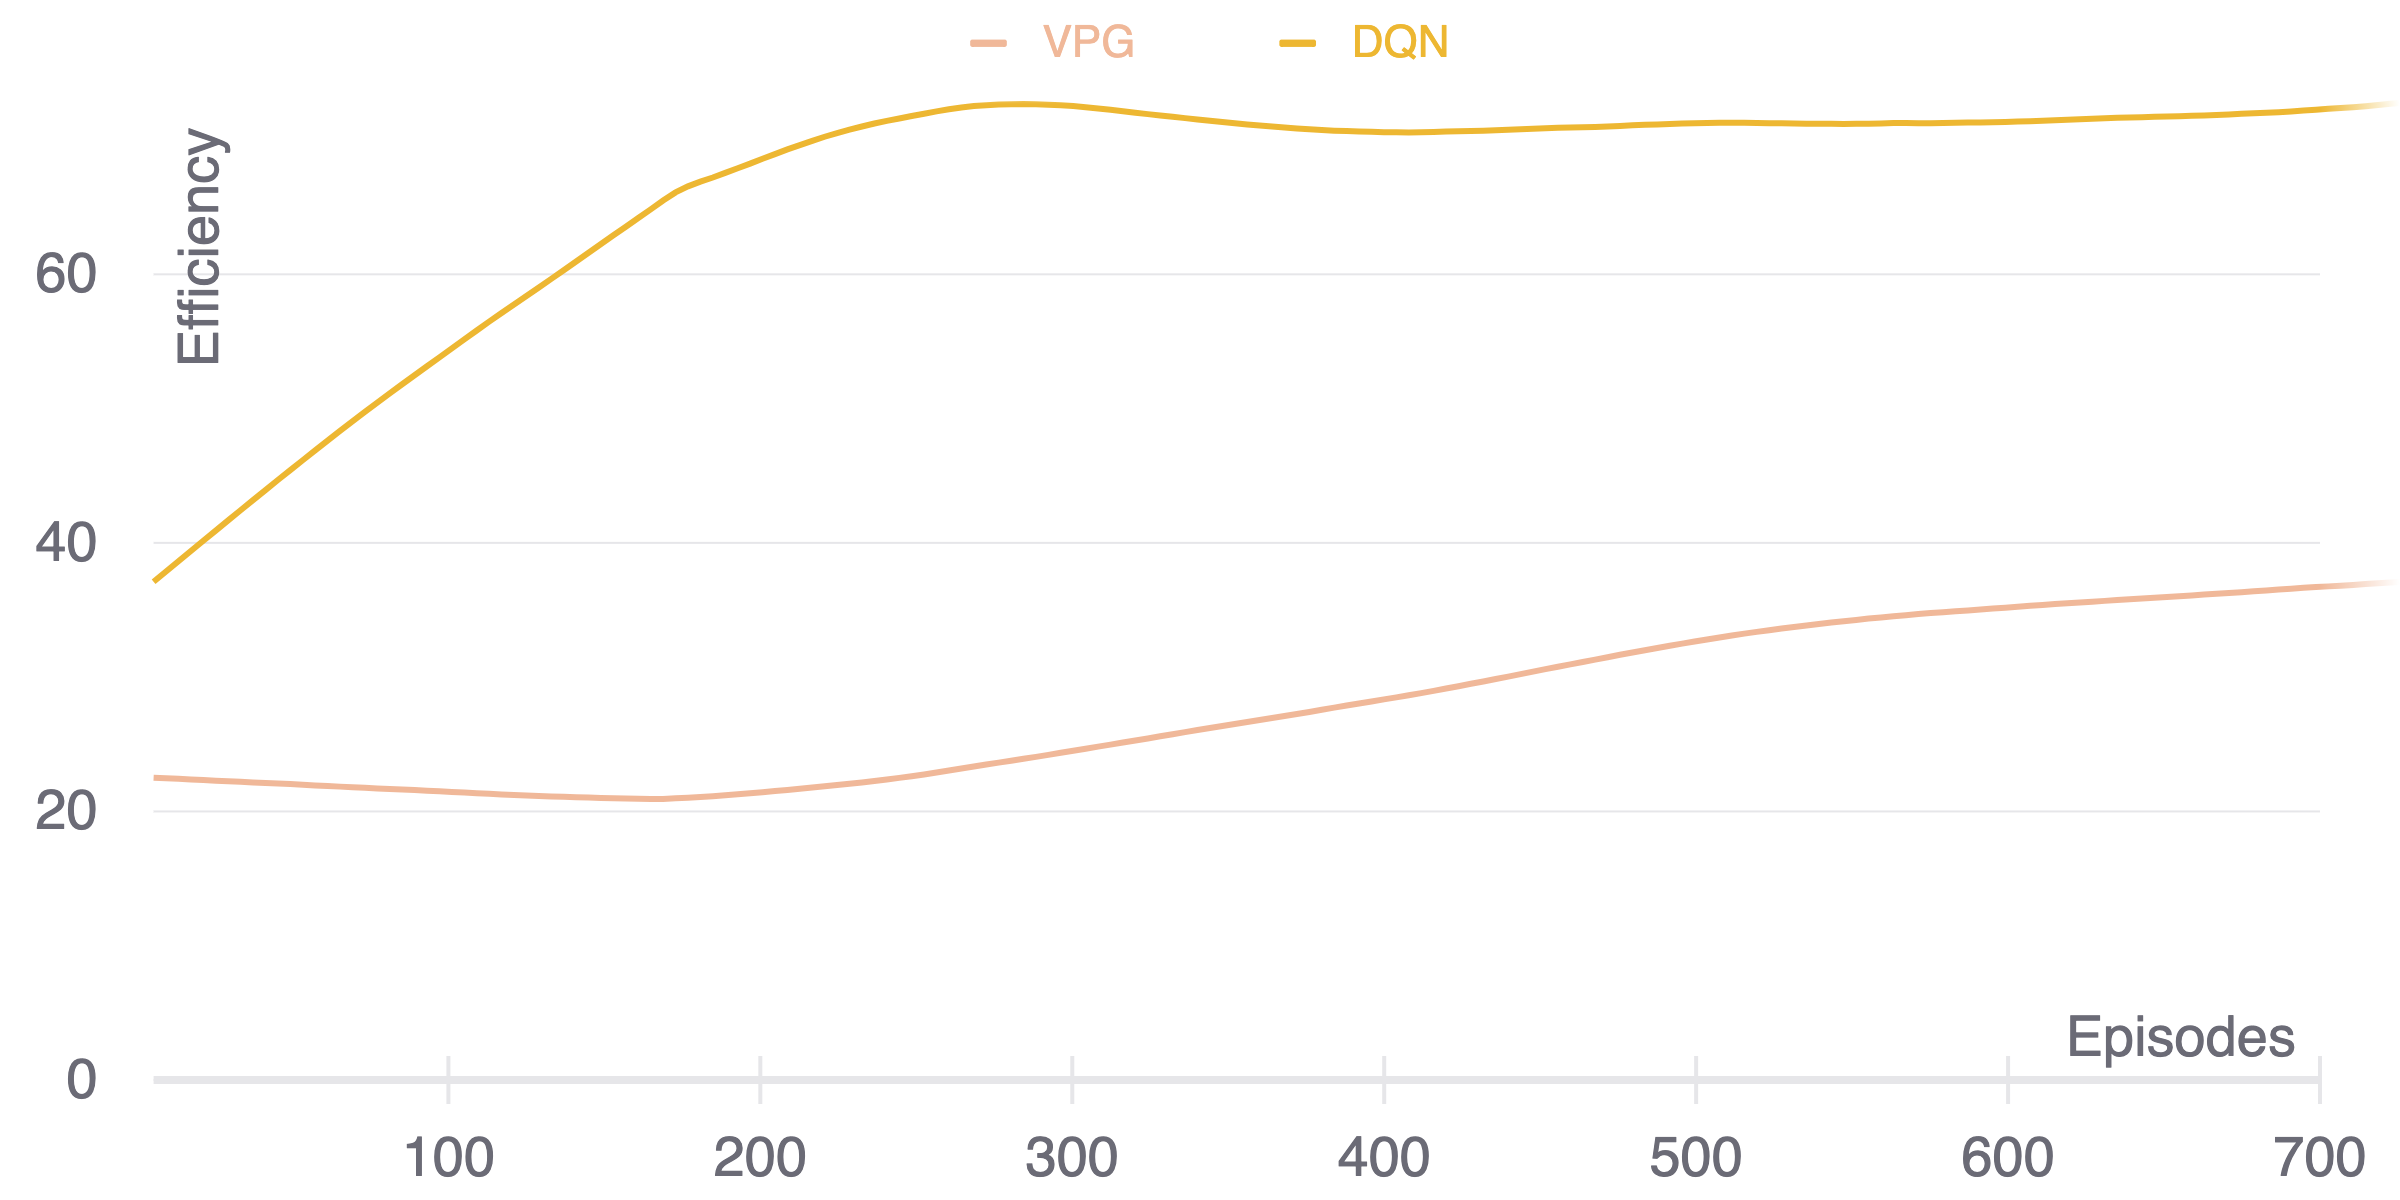
\includegraphics[width=\textwidth]{../assets/dqn-vpg-rllib-single-efficiency}
  \end{subfigure}
  \hfill
  \begin{subfigure}[b]{0.45\textwidth}
    \centering
    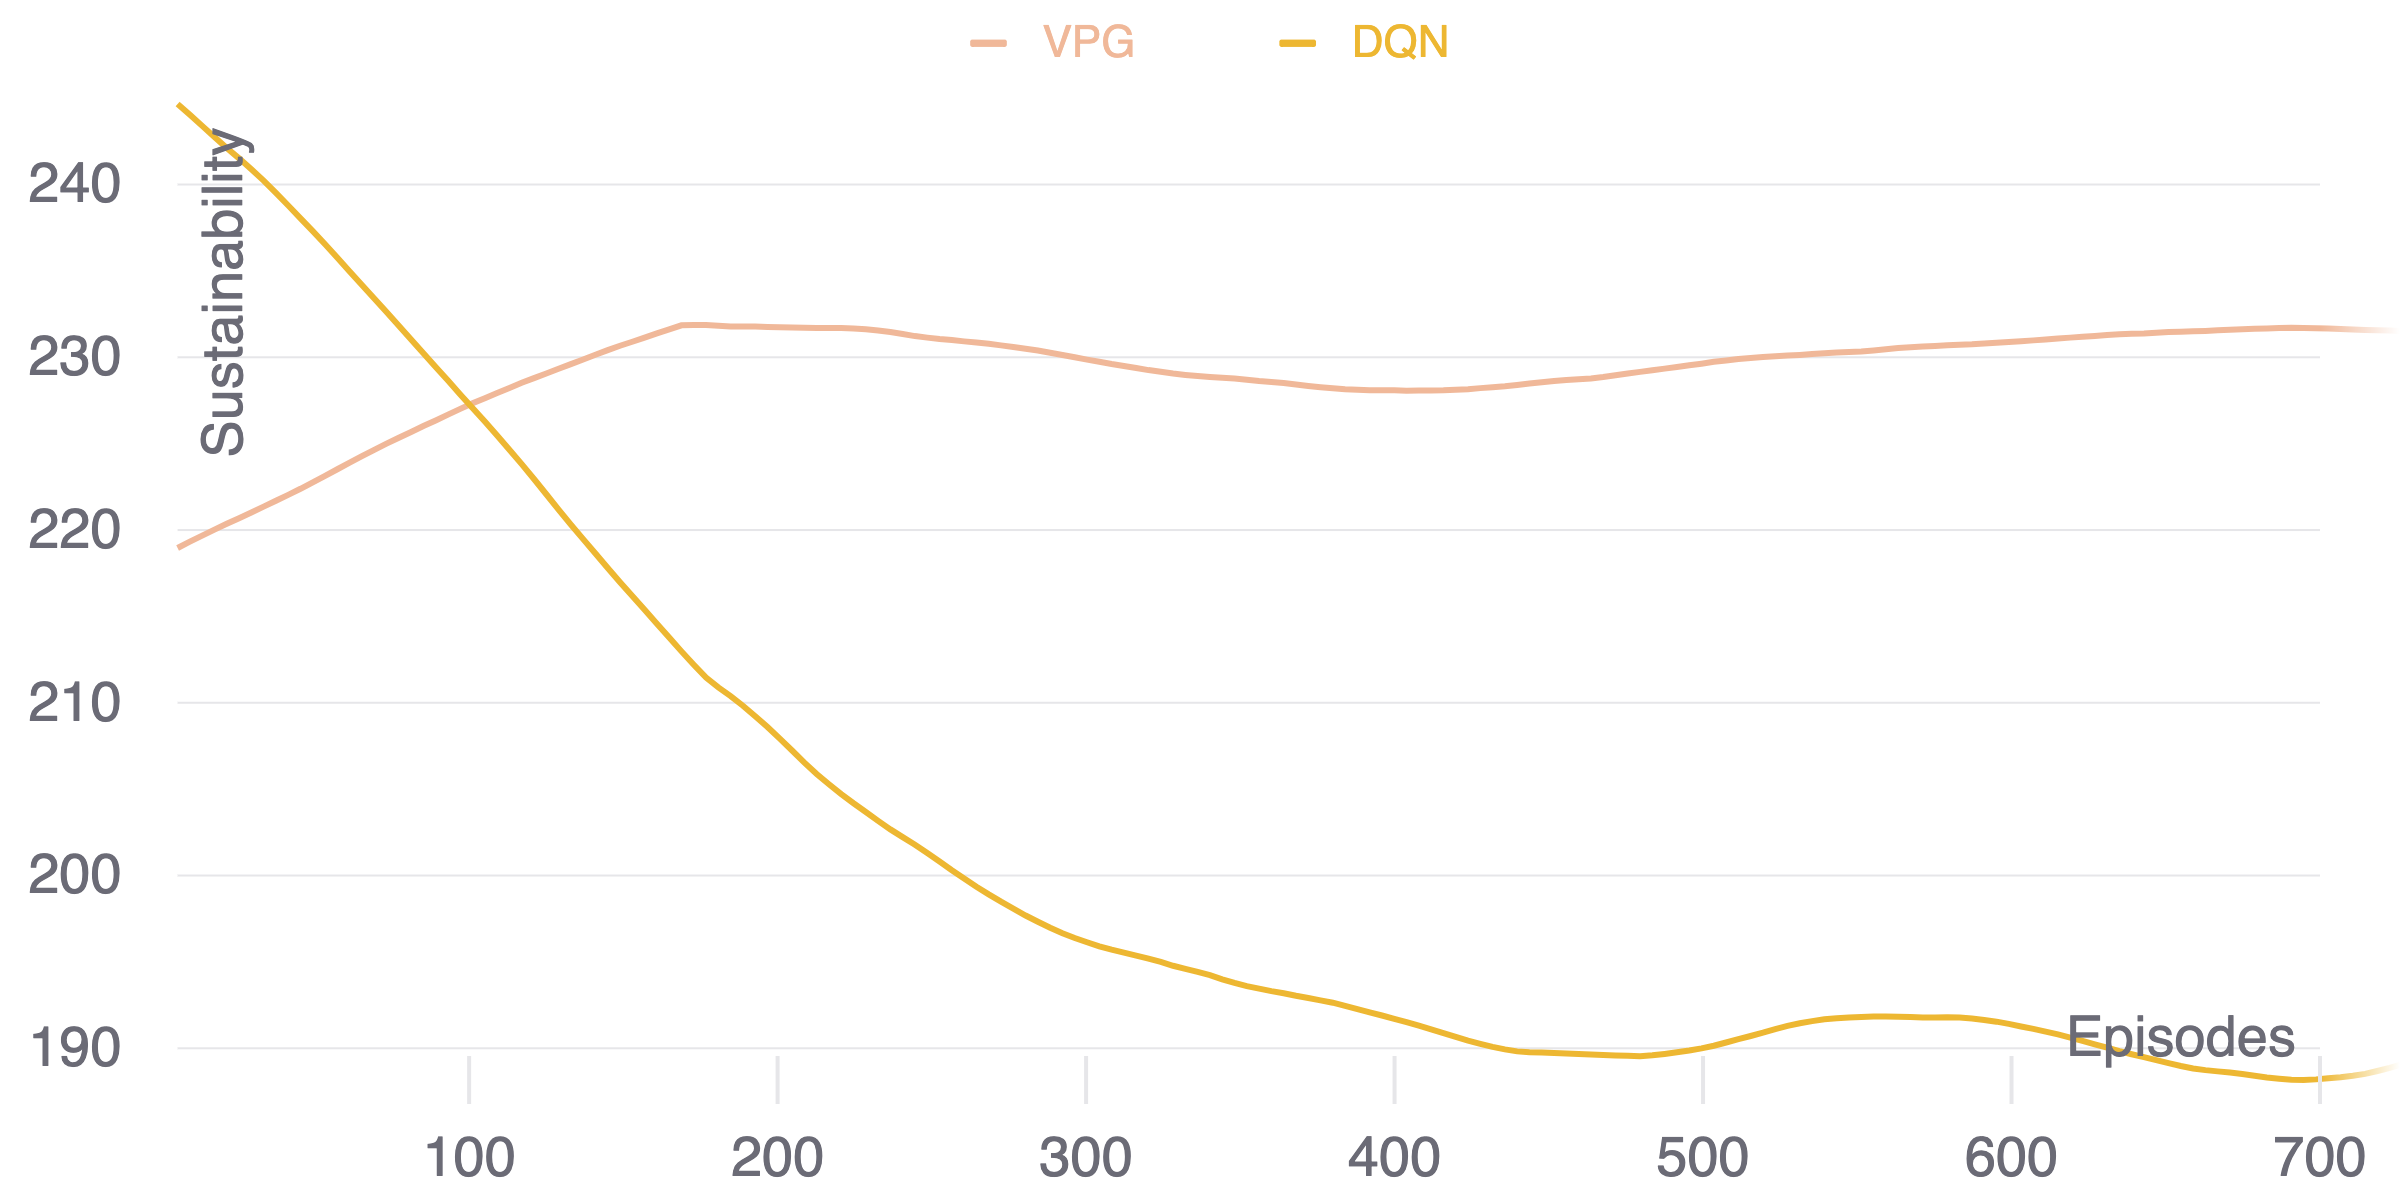
\includegraphics[width=\textwidth]{../assets/dqn-vpg-rllib-single-sustainability}
  \end{subfigure}
  \caption{DQN vs VPG single-agent with RLlib on Harvest}
  \label{fig:dqn-vs-vpg-rllib}
\end{figure}

The outcome of such experiments shows that value-based methods (w.r.t. policy gradient ones) seem more suited for the Harvest environment.

\subsection{Custom VPG vs TRPO vs PPO on Cartpole}
Before running our experiments on the commons game, we test our custom algorithms on a popular environment known as Cartpole: the official description of such environment goes as follows. A pole is attached by an un-actuated joint to a cart, which moves along a frictionless track. The system is controlled by applying a force of $+1$ or $-1$ to the cart. The pendulum starts upright, and the goal is to prevent it from falling over. A reward of $+1$ is provided for every timestep that the pole remains upright. The episode ends when the pole is more than $15$ degrees from vertical, or the cart moves more than $2.4$ units from the center. The problem is considered as solved when the agent is able to obtain an average reward of $195$ over $100$ consecutive trials.

\begin{figure}[h]
  \centering
  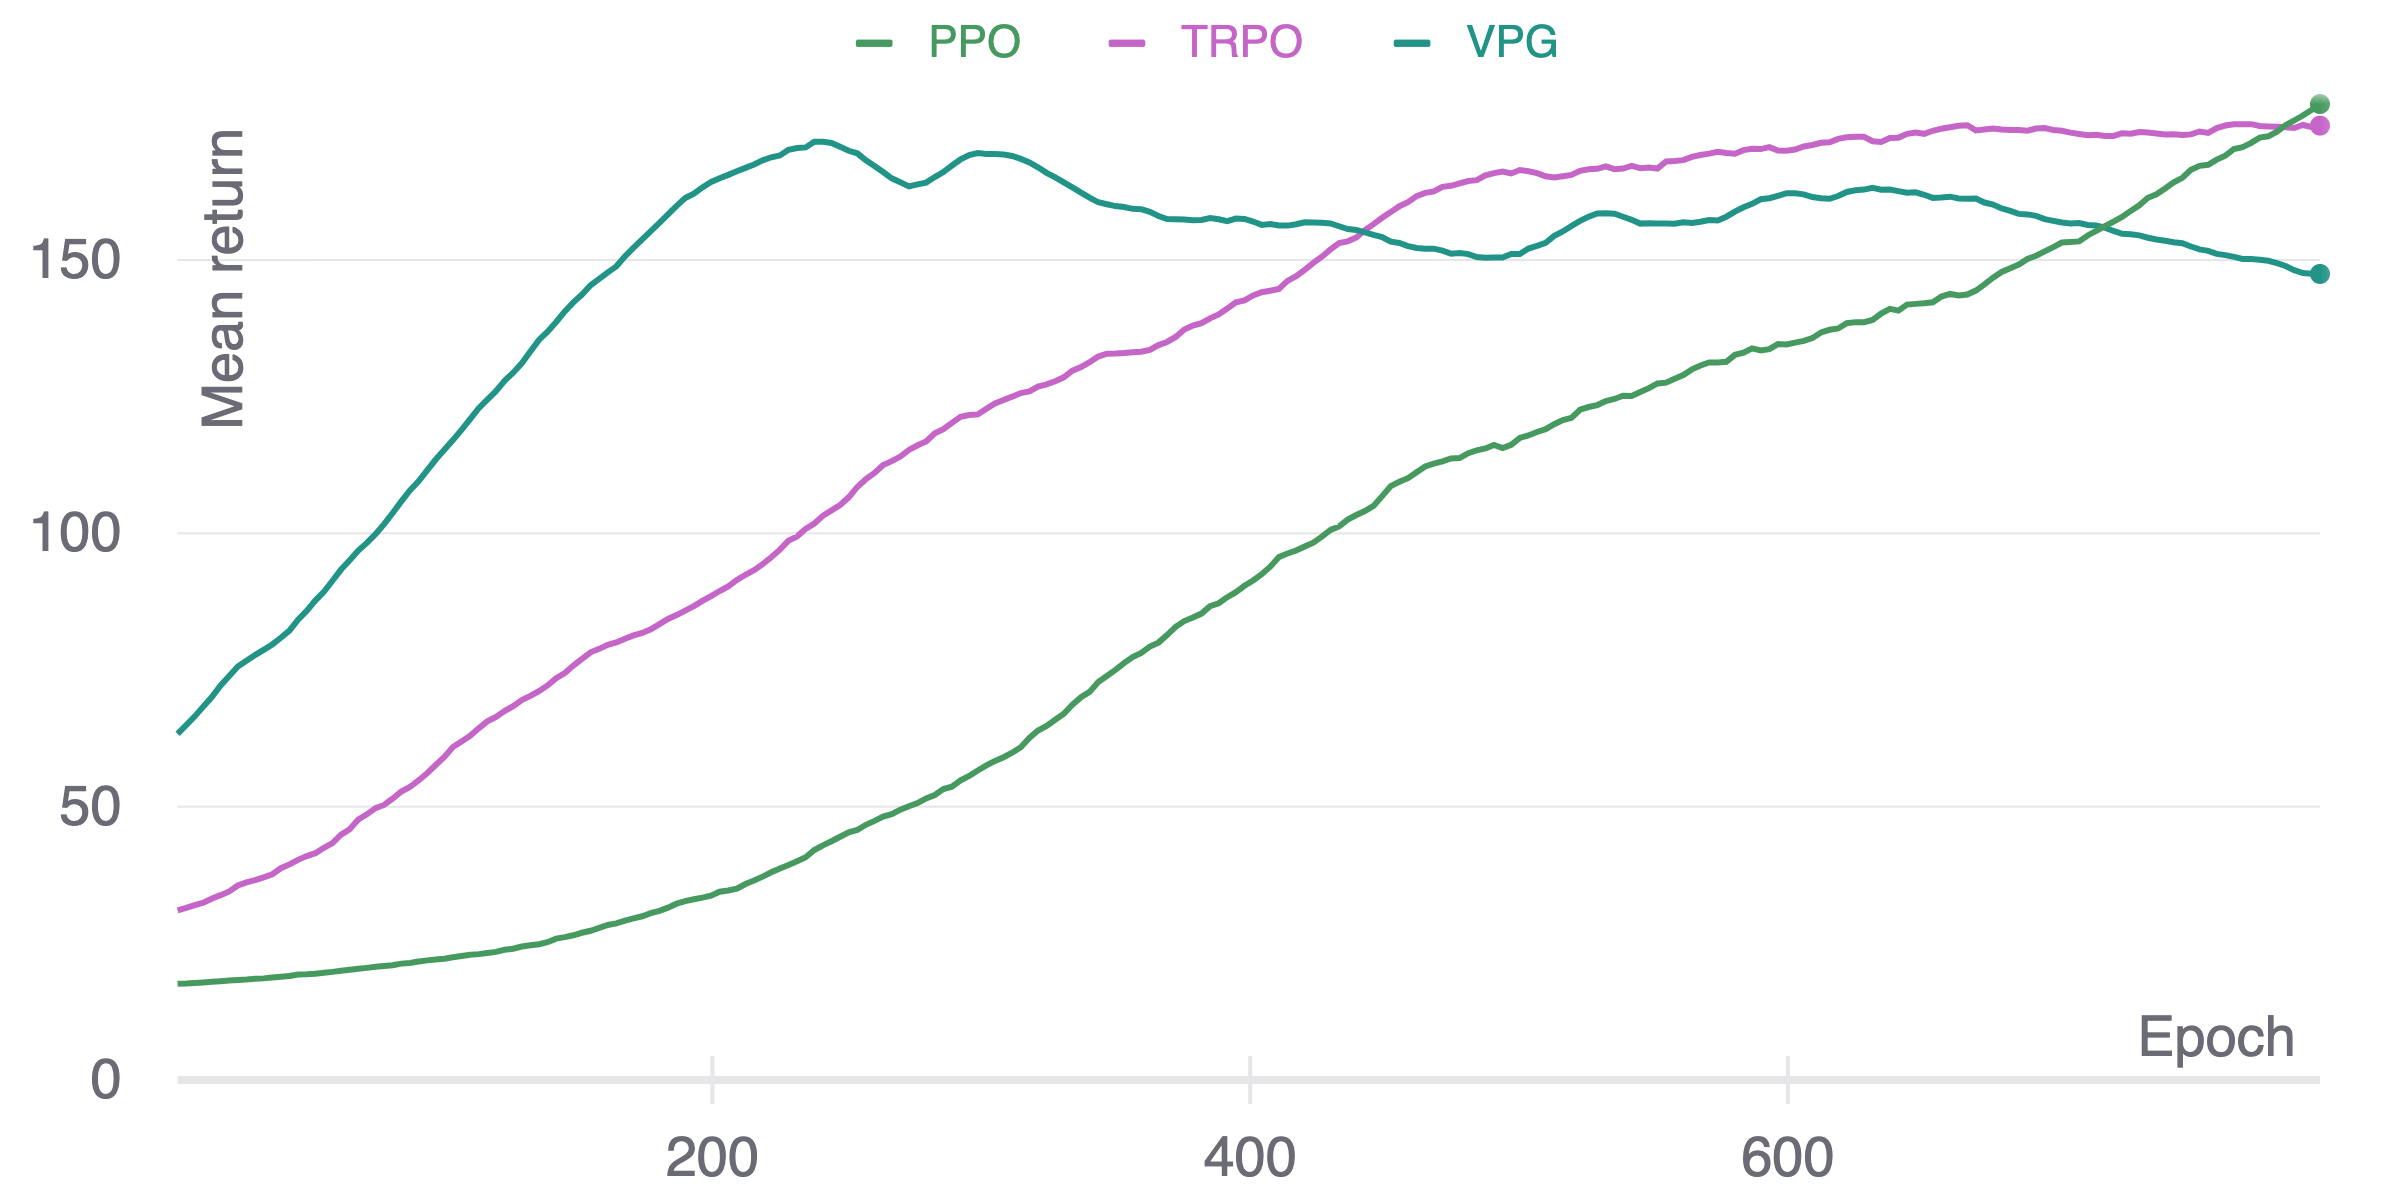
\includegraphics[width=0.7\textwidth]{../assets/cartpole-pg-return}
  \caption{Custom VPG vs TRPO vs PPO on Cartpole}
  \label{fig:cartpole-pg-return}
\end{figure}

Figure \ref{fig:cartpole-pg-return} shows a comparison of VPG, TRPO and PPO on the Cartpole environment, with a number of training epochs equal to $800$. Results reveal that VPG tends to converge faster to higher returns, at the cost of a very high variance (both in returns and in the loss), while both TRPO and PPO achieve better results than PPO, but their learning curves are a bit steeper. 

The main outcome of this experiment is that our custom implementations are valid, as agents are able to learn effectively in the selected test environment.

\subsection{Custom VPG vs TRPO vs PPO on single-agent Harvest}
This experiment tests how our custom algorithms compare with each other on the commons game, with just a single agent and $1000$ training epochs. Figure \ref{fig:vpg-trpo-ppo-single} shows that both VPG and PPO converge to similar average returns (close to the ones obtained with RLlib's implementation of VPG, as reported in figure \ref{fig:dqn-vs-vpg-rllib}). Moreover, we can observe that TRPO diverges to worse efficiencies $U$ during training, while on the Cartpole environment it performed on par with both VPG and PPO. This could be explained by the choice of hyperparameters, which could be optimized by some kind of search in the parameter space, such as grid search: unfortunately, such computations are costly in terms of resource requirements and we leave them for future improvements.

\begin{figure}
  \centering
  \begin{subfigure}[b]{0.45\textwidth}
    \centering
    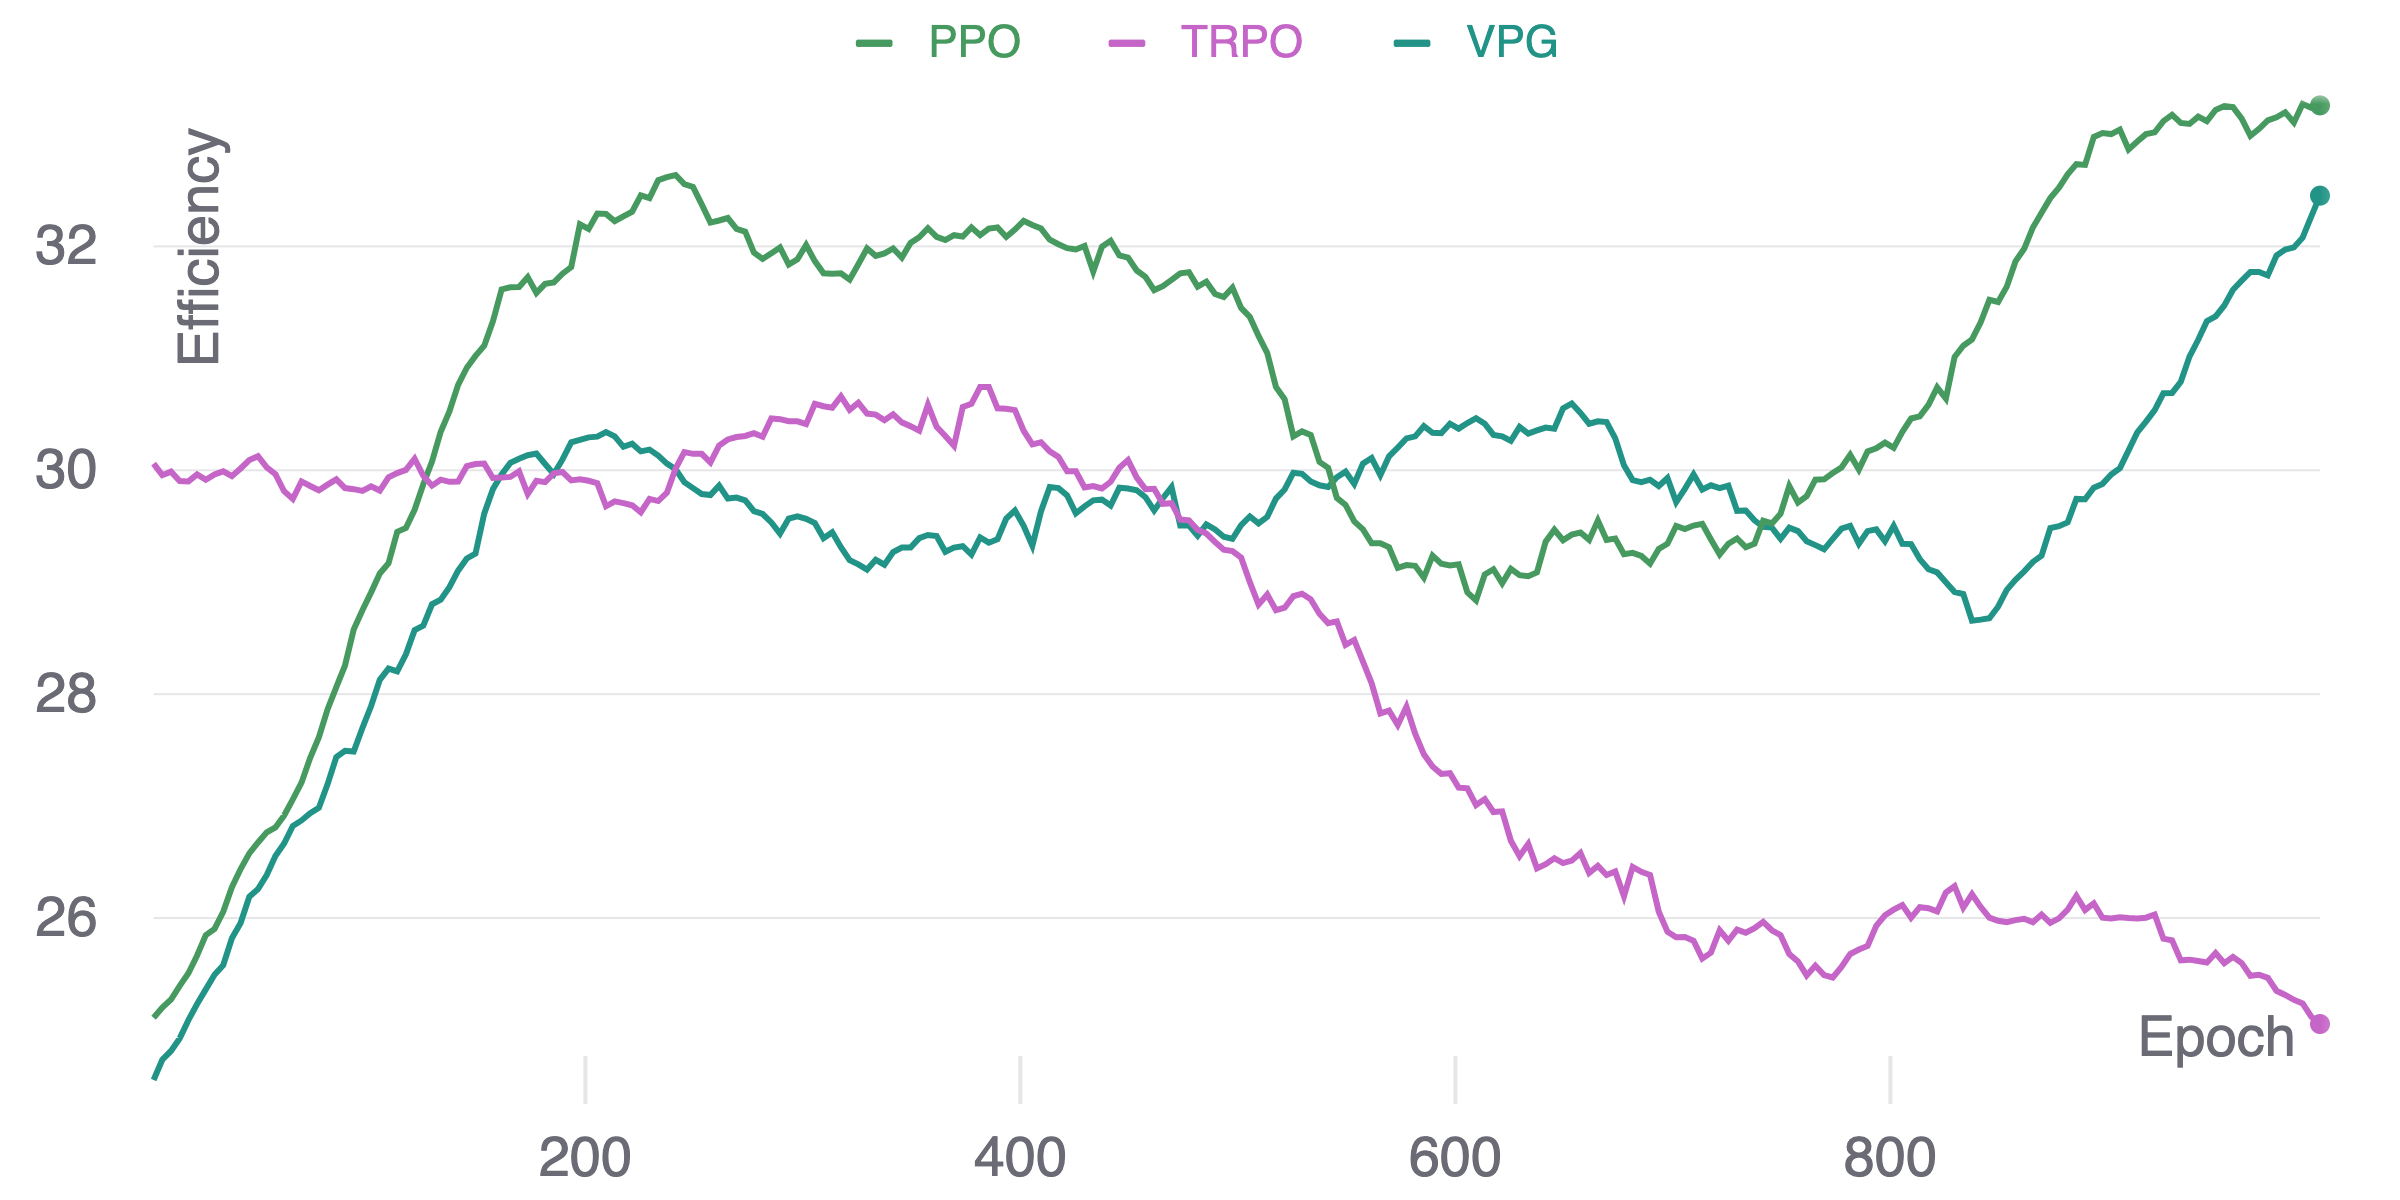
\includegraphics[width=\textwidth]{../assets/vpg-trpo-ppo-single-efficiency}
  \end{subfigure}
  \hfill
  \begin{subfigure}[b]{0.45\textwidth}
    \centering
    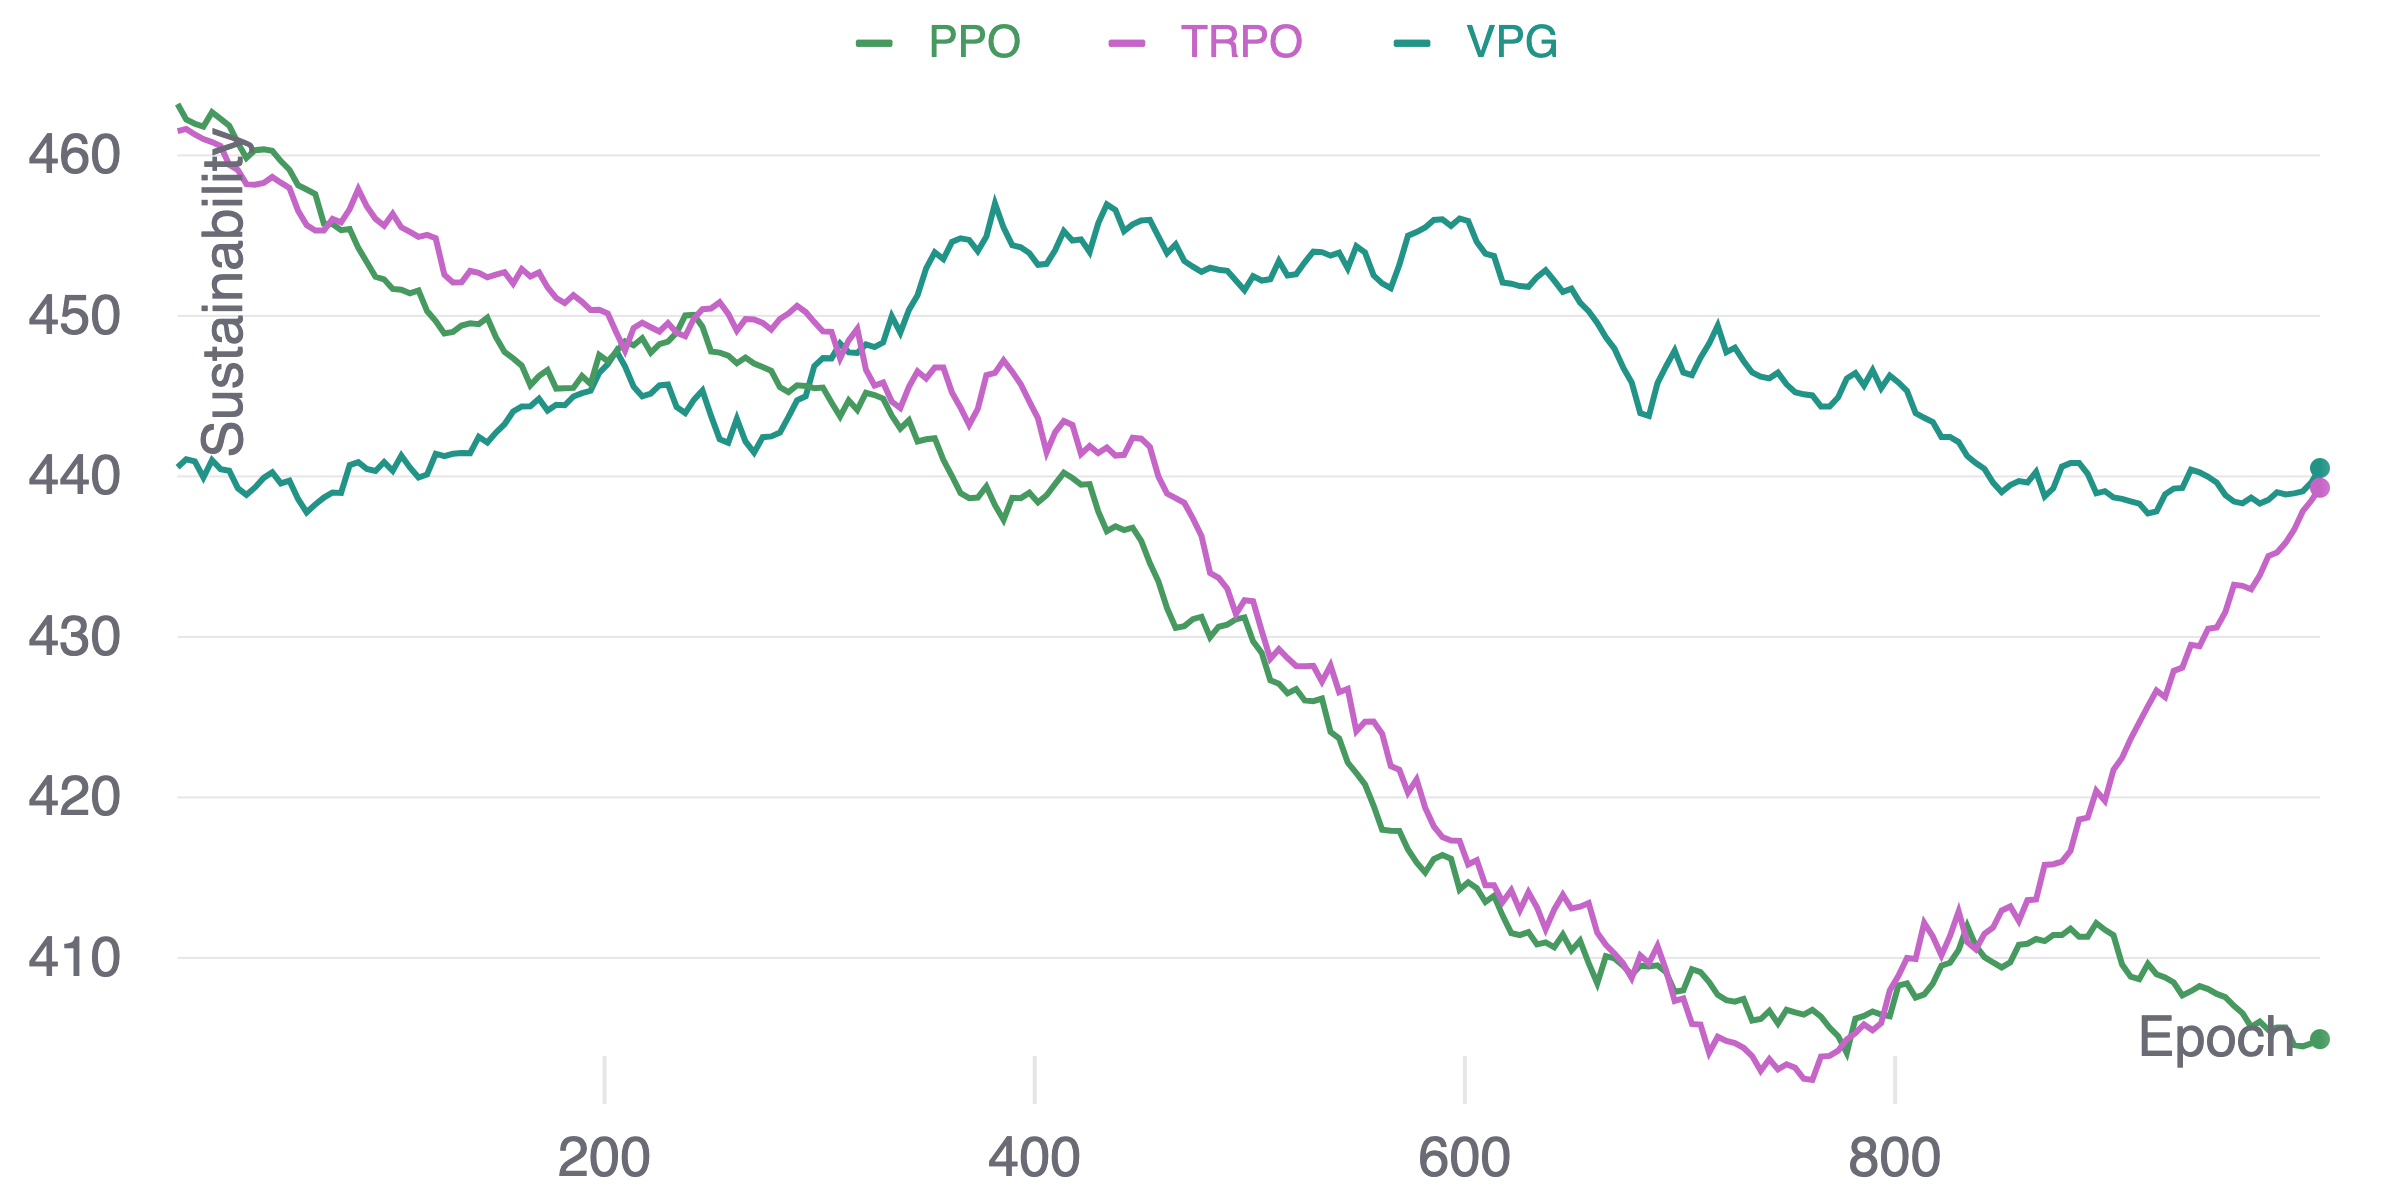
\includegraphics[width=\textwidth]{../assets/vpg-trpo-ppo-single-sustainability}
  \end{subfigure}
  \caption{Custom single-agent VPG vs TRPO vs PPO on Harvest}
  \label{fig:vpg-trpo-ppo-single}
\end{figure}

\subsection{Custom PPO on multi-agent Harvest}
In order to test our Social Learning strategy and understand whether cooperation improves or deteriorates social outcome metrics on the Harvest enviroment, we compare two training runs with and without the gifting action enabled. Moreover, we also compare two other experiments with the Replenishable and Fixed Budget gifting strategies, to observe their performance. Given the computational complexity of the Harvest environment in a multi-agent scenario, running experiments for the same number of episodes used in the original paper is prohibitive and would require more resources than available at the time of writing: thus, we limit ourselves to $500$ epochs or fewer and observe outcomes up to that point. 

\begin{figure}[h]
  \centering
  \begin{subfigure}[b]{0.3\textwidth}
    \centering
    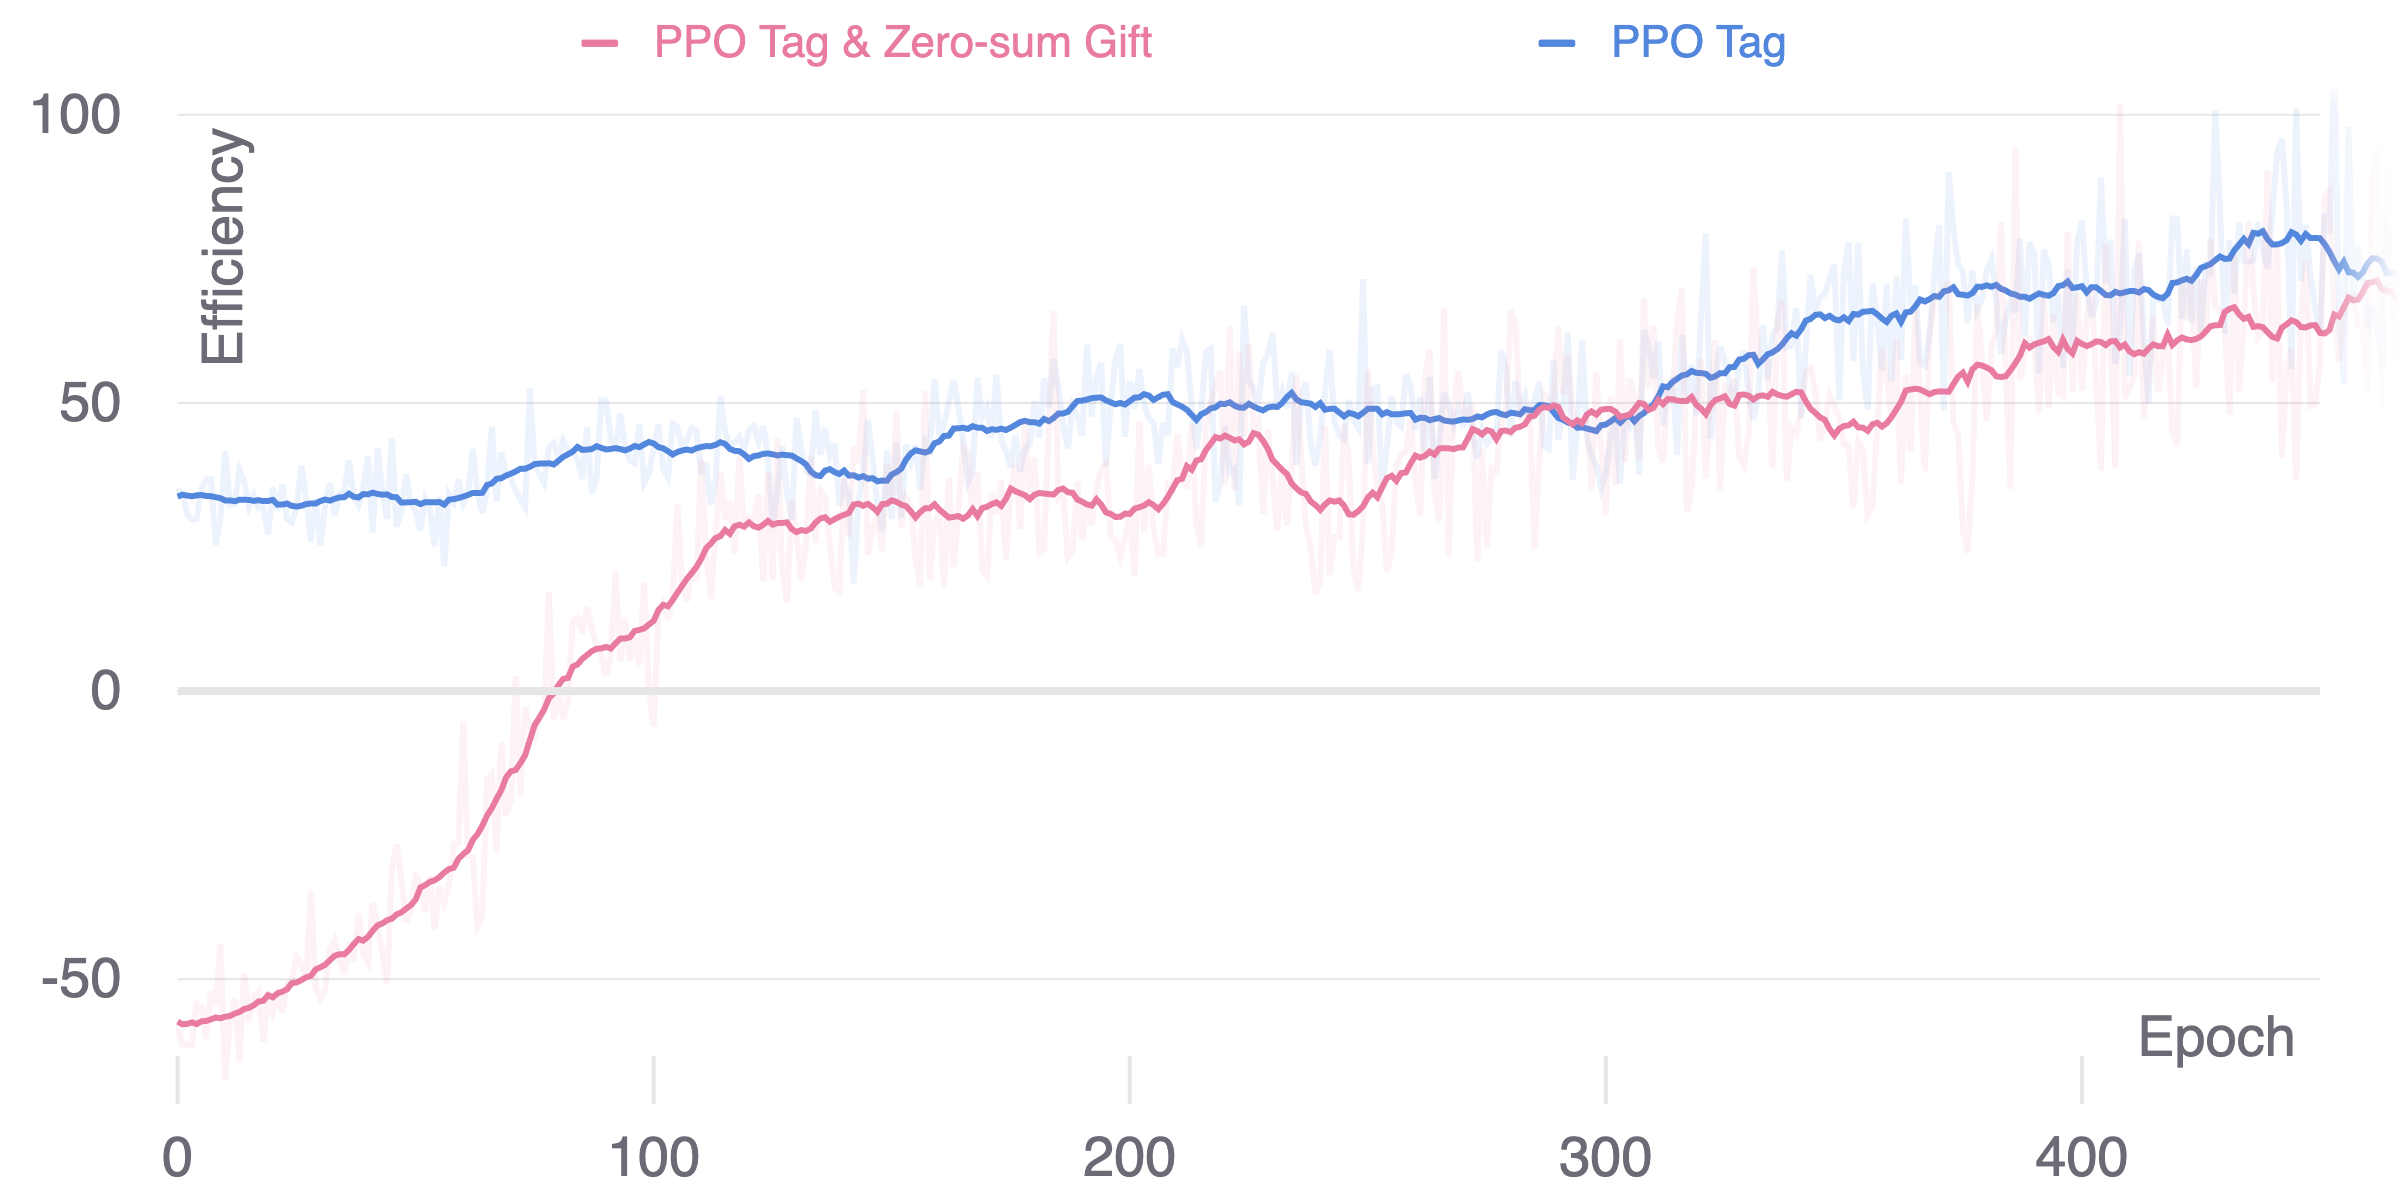
\includegraphics[width=\textwidth]{../assets/ppo-tag-gift-vs-nogift-efficiency}
  \end{subfigure}
  \hfill
  \begin{subfigure}[b]{0.3\textwidth}
    \centering
    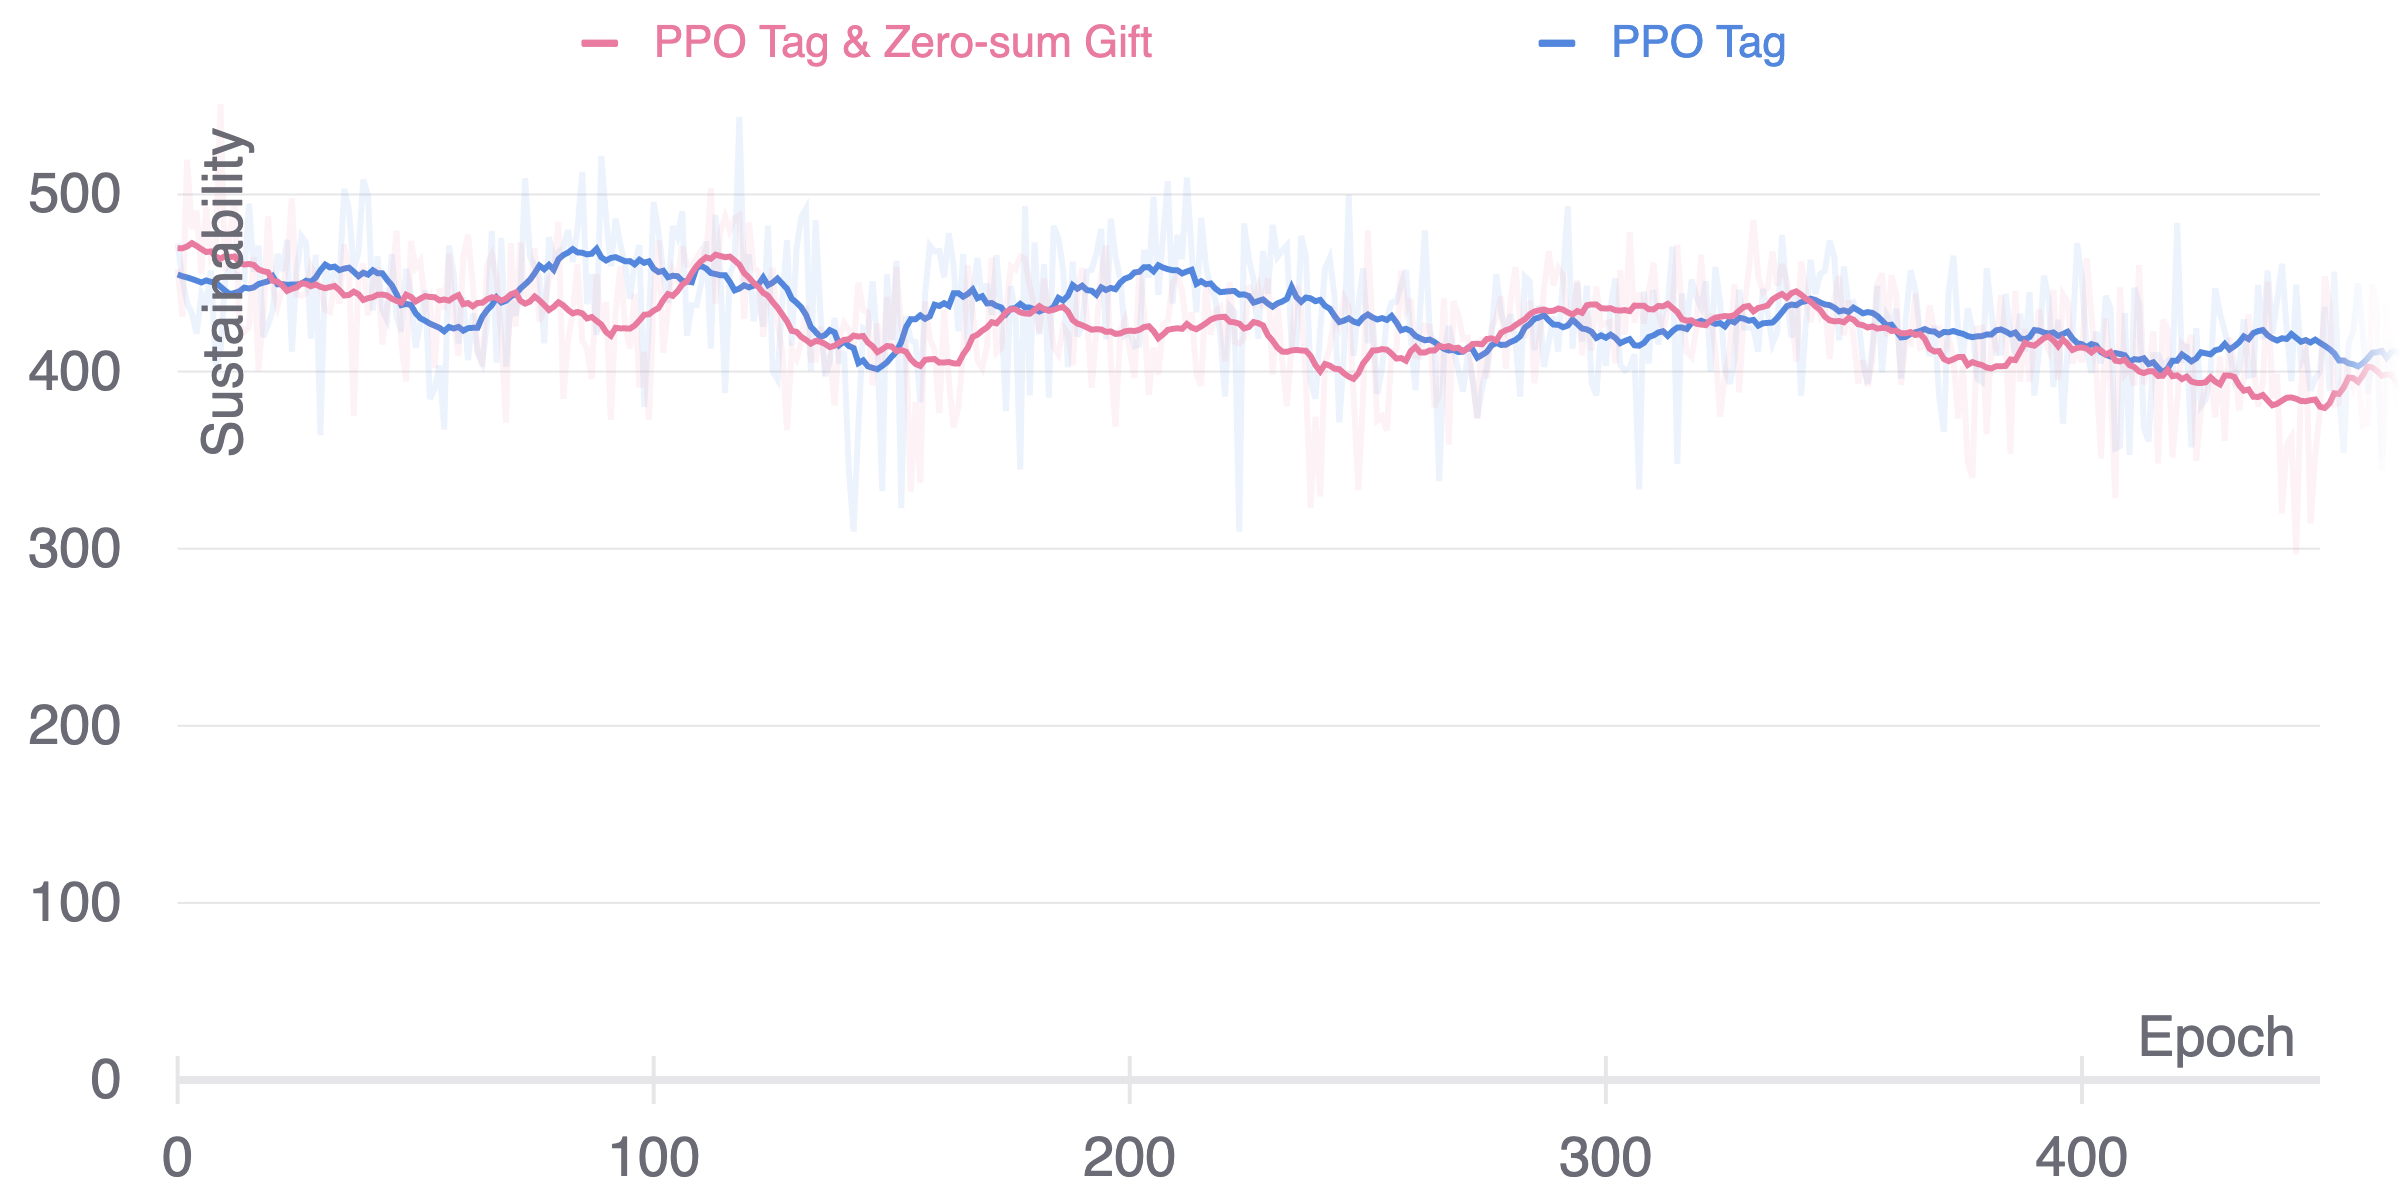
\includegraphics[width=\textwidth]{../assets/ppo-tag-gift-vs-nogift-sustainability}
  \end{subfigure}
  \hfill
  \begin{subfigure}[b]{0.3\textwidth}
    \centering
    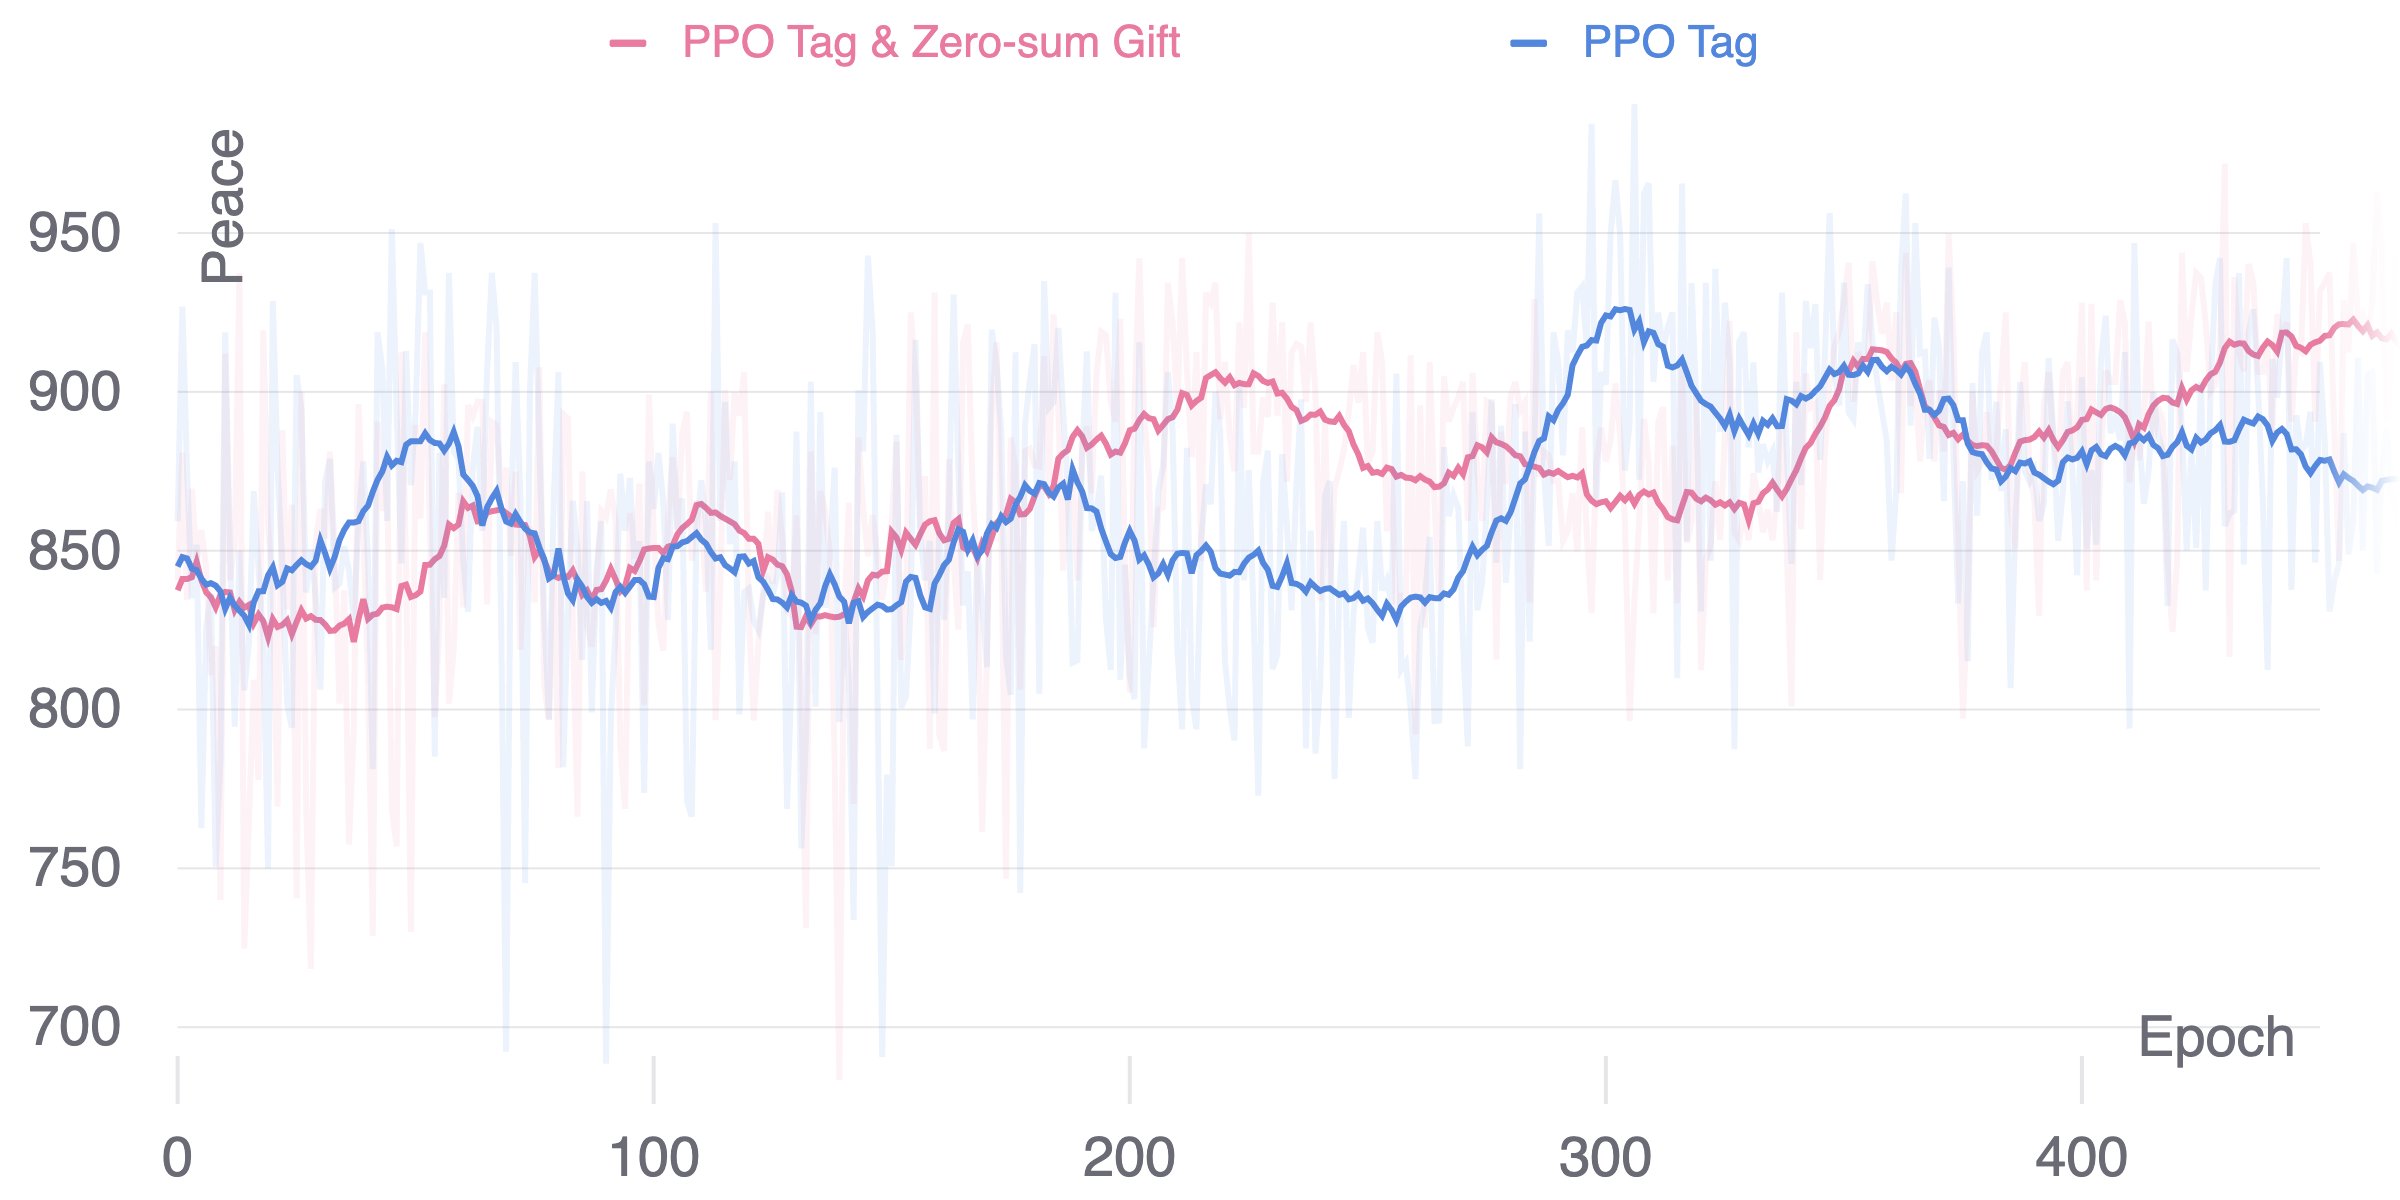
\includegraphics[width=\textwidth]{../assets/ppo-tag-gift-vs-nogift-peace}
  \end{subfigure}
  \caption{Custom multi-agent PPO on Harvest, with and without Zero-Sum gifting}
  \label{fig:ppo-gift-nogift}
\end{figure}

Figure \ref{fig:ppo-gift-nogift} shows social outcome metrics for $4$ agents trained both without any gifting whatsoever and with the Zero-Sum gifting mechanism, which revelead to be the one giving best results on the original paper \cite{gifting}. Both training runs had the tagging action enabled and lasted for around $500$ epochs, all hyperparameters being the same. Results show that agents tend to be very generous during the first few hundred epochs, as their efficiency is inclined on the negative side, meaning that there is more gifting than collecting. Later training stages show that agents with and without gifting tend to converge to similar outcomes, but those without the possibility to gift do so in a faster way. 

\begin{figure}[h]
  \centering
  \begin{subfigure}[b]{0.3\textwidth}
    \centering
    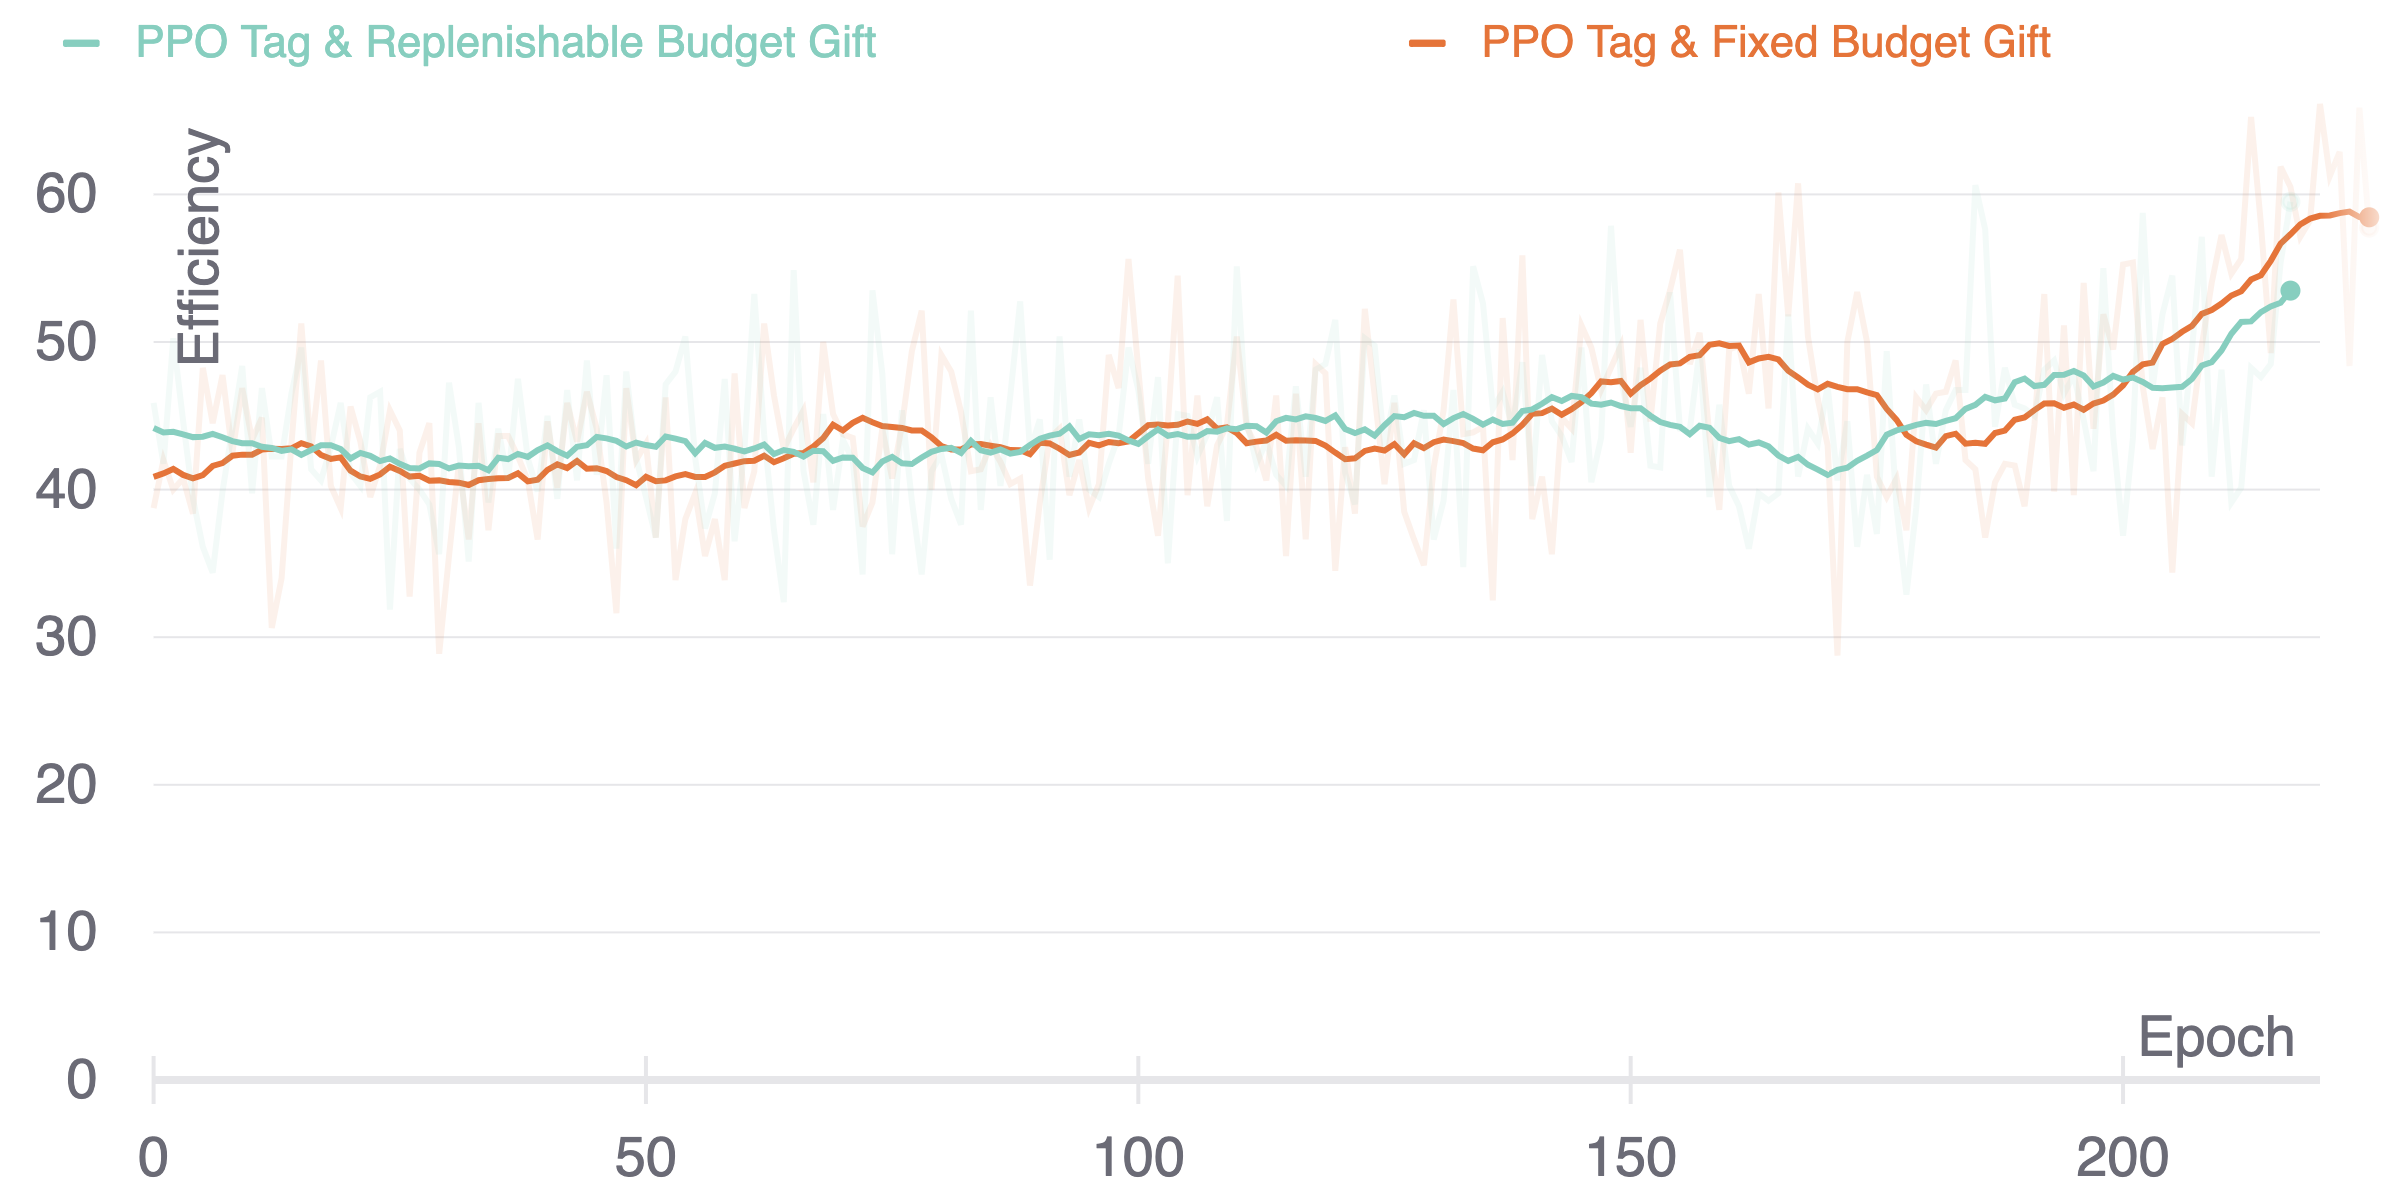
\includegraphics[width=\textwidth]{../assets/ppo-gifting-fixed-vs-replenishable-efficiency}
  \end{subfigure}
  \hfill
  \begin{subfigure}[b]{0.3\textwidth}
    \centering
    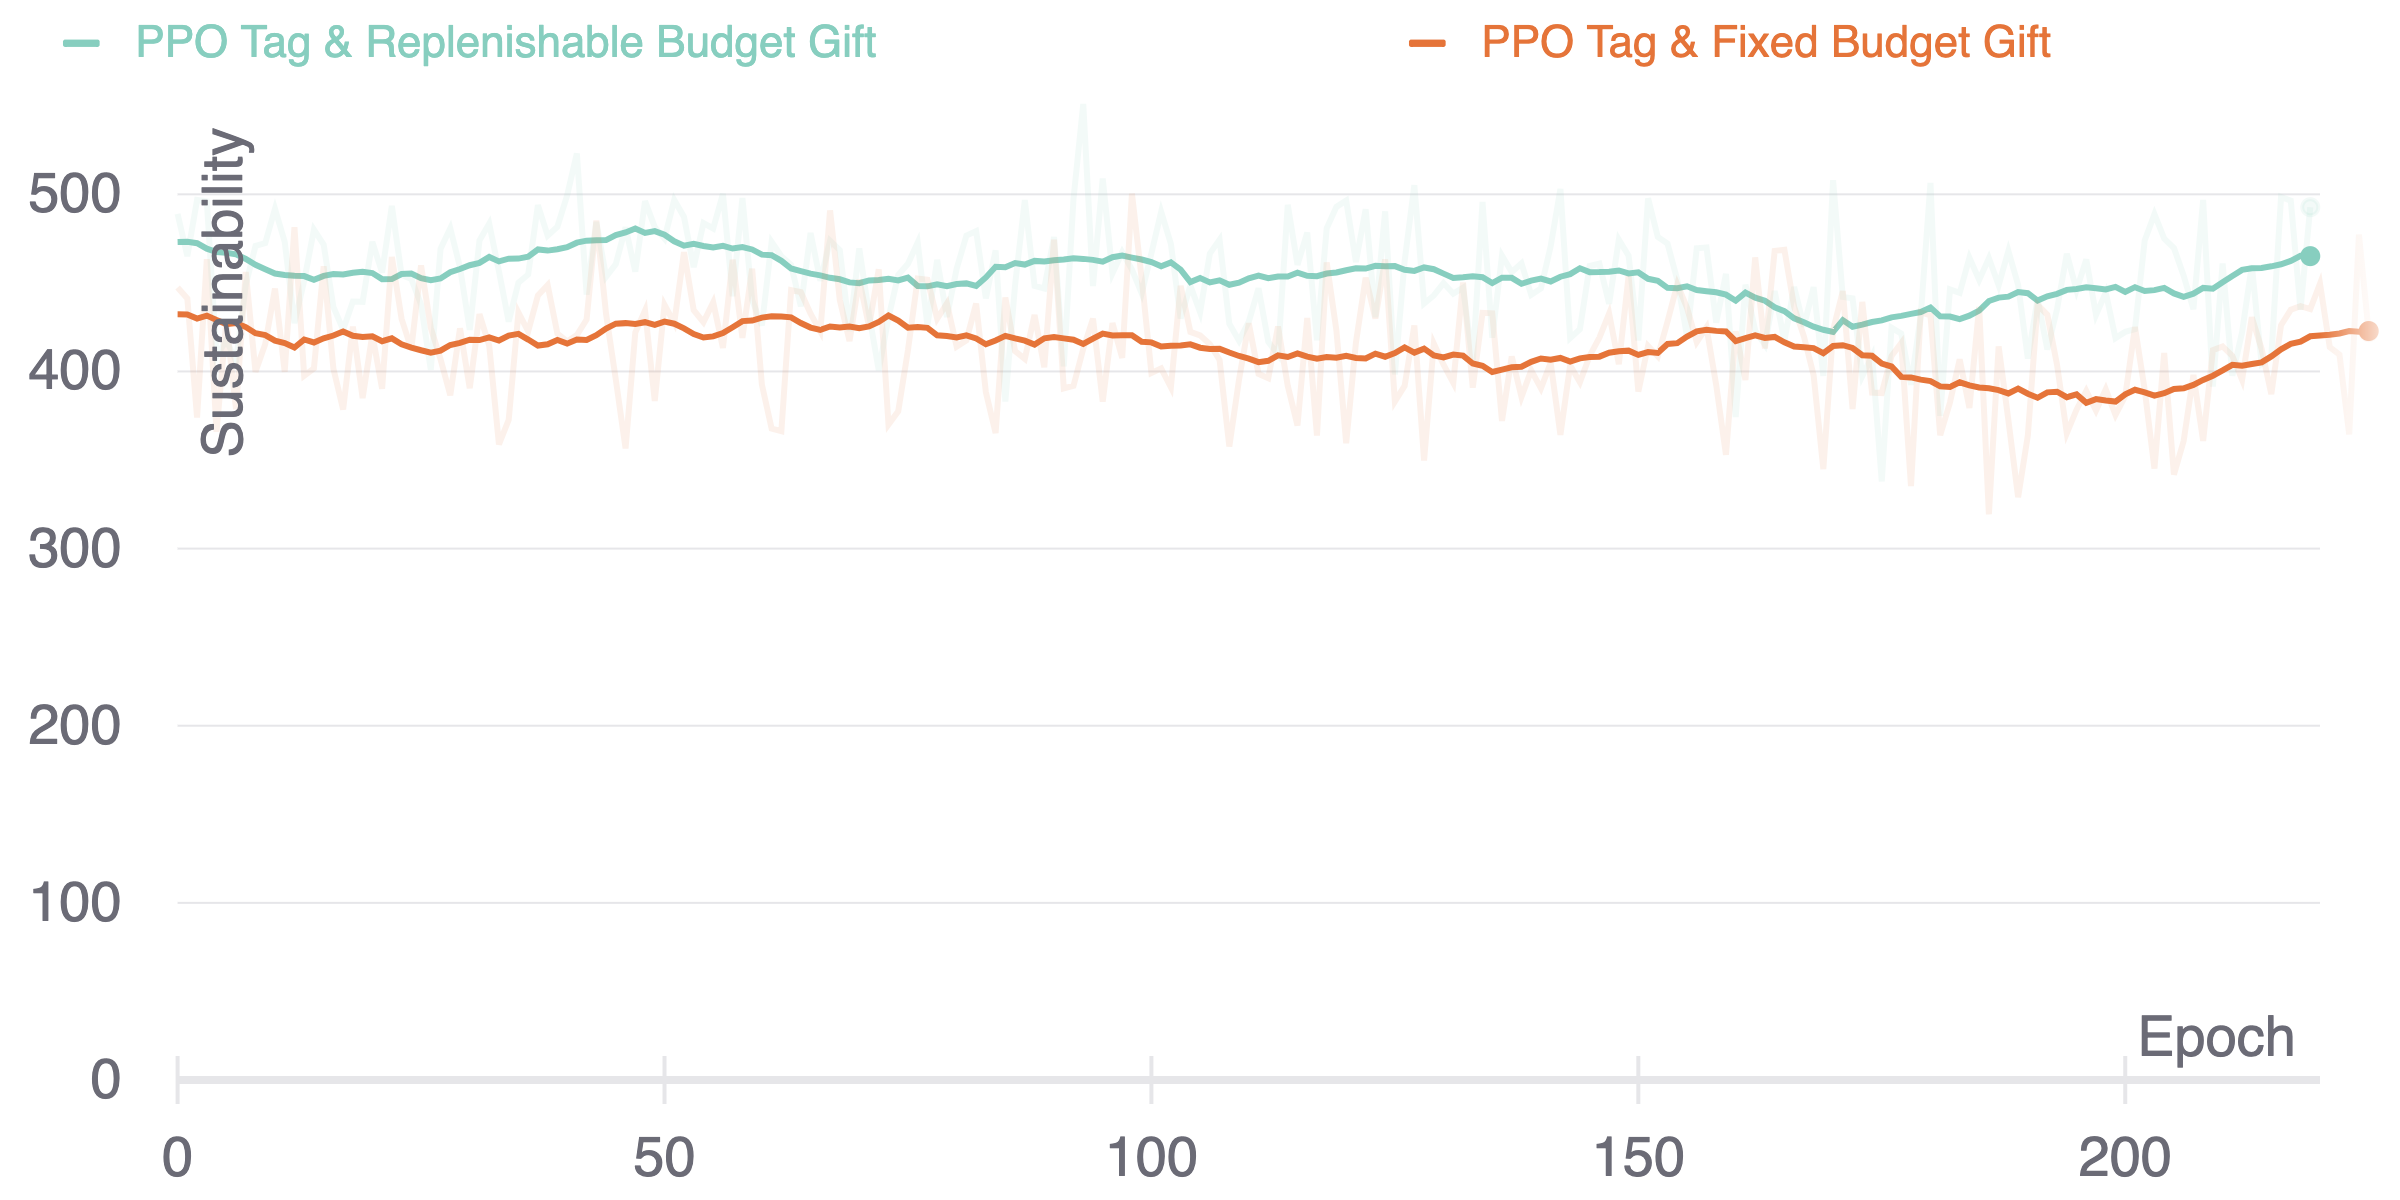
\includegraphics[width=\textwidth]{../assets/ppo-gifting-fixed-vs-replenishable-sustainability}
  \end{subfigure}
  \hfill
  \begin{subfigure}[b]{0.3\textwidth}
    \centering
    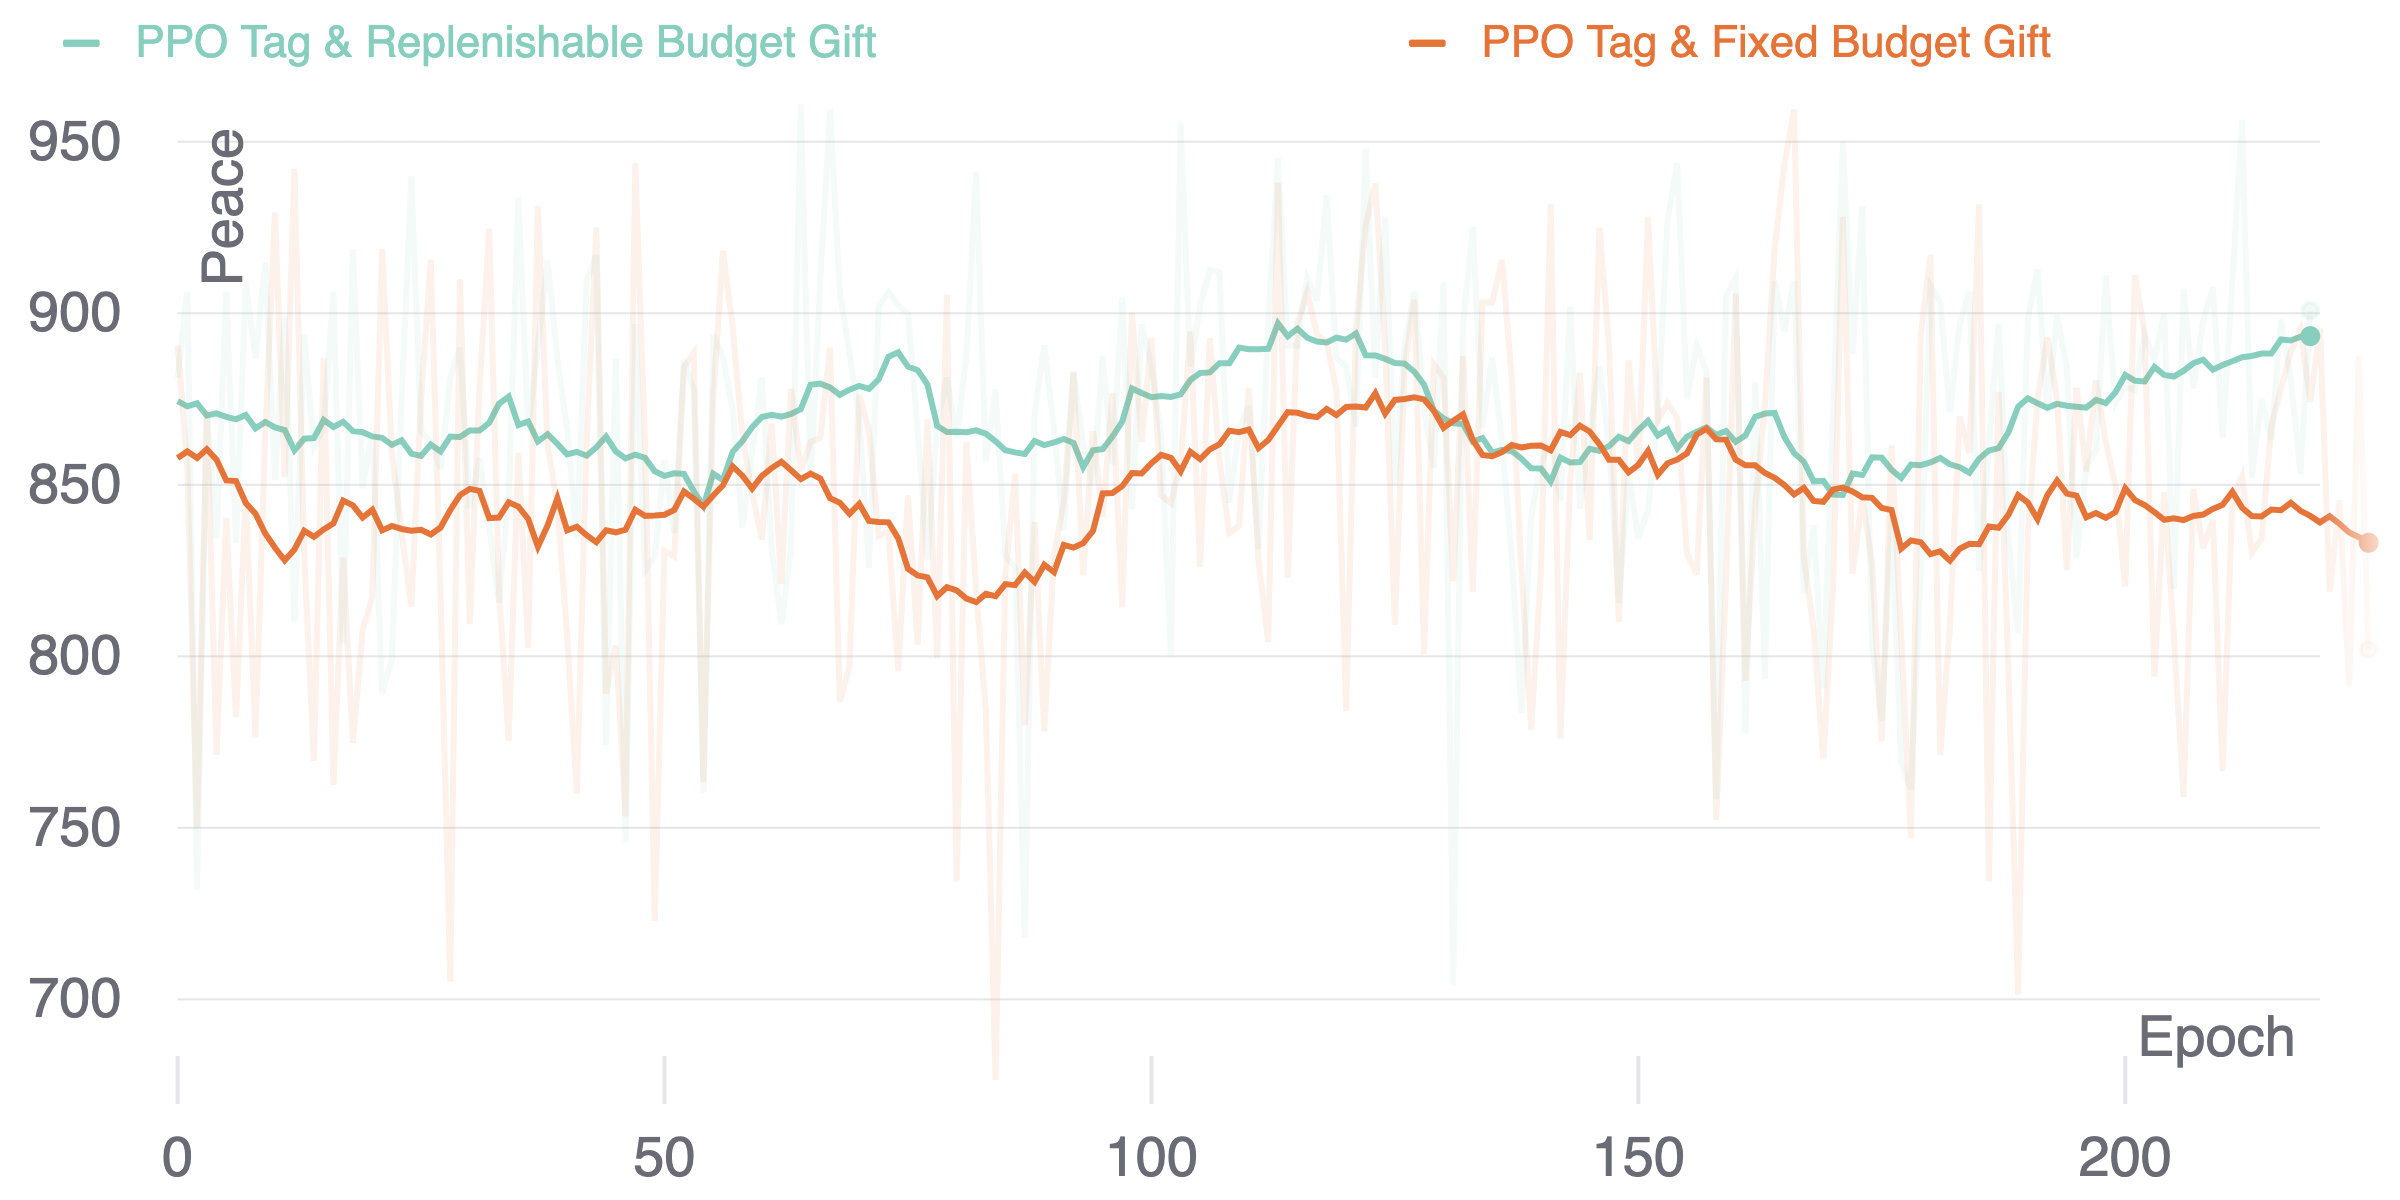
\includegraphics[width=\textwidth]{../assets/ppo-gifting-fixed-vs-replenishable-peace}
  \end{subfigure}
  \caption{Custom multi-agent PPO on Harvest, with Replenishable and Fixed Budget gifting}
  \label{fig:ppo-gift-replenishable-fixed}
\end{figure}

Figure \ref{fig:ppo-gift-replenishable-fixed} shows social outcome metrics for $4$ agents trained with the Replenishable Budget gifting strategy and with the Fixed Budget mechanism. Both training runs had the tagging action enabled and lasted for around $250$ epochs, all hyperparameters being the same. Results show that both gifting strategies tend to converge to similar outcomes.

\newpage
\section{Conclusions}
In this work we implemented the popular Harvest environment from scratch, to make it compatible with the OpenAI Gym API. Then, we checked the correctness of the environment by leveraging RLlib's DQN in a single-agent setting and observed convergence. Moreover, we implemented three policy gradient algorithms, namely VPG, TRPO (with regularizion rather than exact constrained methods) and PPO. To test our custom models we compared our VPG implementation with RLlib's one in a single-agent setting on the custom Harvest environment and observed similar outcomes. With this experiment we also observed that VPG obtained much lower results w.r.t. DQN, in terms of mean returns. The last contribution is related to the implementation of a Social Learning scheme called gifting, in which agents can give some of their rewards to other agents. Supposedly, such technique should enable cooperation between agent and foster a collective behavior. Unfortunately, as in the original paper, we didn't obtain better social outcome metrics on a multi-agent scenario with gifting than without. One difference that we observed w.r.t. the original paper is that agents with Zero-Sum gifting tend to converge slower w.r.t. agents without the possibility to gift, which is the exact opposite outcome w.r.t. what authors reported in \cite{gifting}. Our final remark is that, even though policy gradient methods should theoretically perform best with stochastic processes (such as Harvest with local observations), empirical results show that value-based method tend to achieve better outcomes.


\newpage
\bibliography{references}

\newpage
\appendix

\section{Reinforcement Learning setting}
\label{appendix:rl}
This section introduces theoretical foundations of both value-based methods and policy gradient techniques at a broad level.

\subsection{Value-based methods}
Value-based methods only store a value function (usually the state-action function $Q$), instead of explicitly storing the policy. Actions are then derived from the value function by picking the one with the best value. One of the most popular value-based algorithms is $Q$-learning and its neural variant DQN: a DQN (Deep $Q$-Network) \cite{dqn} leverages neural networks from the point of view of universal function approximators, to estimate the optimal $Q^*$ state-action function. The main idea behind DQN is to estimate $Q^*$ with $Q_\theta$ and use the Bellman equation to update the weights $\theta$ of the network so that $Q_\theta\rightarrow Q^*$. In particular, the loss to be used is a regression one (e.g. MSE or Huber) to minimize the so-called TD (Temporal Difference) error:
$$
L(\theta)=\mathbb{E}_{(s_t,a_t,r_{t+1},s_{t+1})}\left[\left(\underbrace{r_{t+1}+\gamma\max_{a_{t+1}}Q_\theta(s_{t+1}, a_{t+1}) - Q_\theta(s_t, a_t)}_{TD}\right)^2\right]
$$

About the network architecture, the literature does not follow a clear definition, so that the term DQN is mostly linked to the whole training pipeline required to reach good estimates of the optimal $Q$ function. For example, in the original paper \cite{dqn} DeepMind researchers use an initial CNN (Convolutional Neural Network), since their input is represented by videogame frames, followed by an MLP (Multi-Layer Perceptron). Instead, the original Harvest implementation \cite{harvest} only relies on the final fully-connected layers, where the number of input neurons is given by the linearization of the selected observation, the number of hidden cells and the number of hidden layers are hyperparameters, while the number of outputs is equal to the size of the action space. 

Another thing to notice is that the weights used for the target versus the current (presumably non-optimal) $Q$ values are different. In practical terms, a separate network is used to estimate the TD target. This target network has the same architecture as the function approximator but with frozen parameters. Every $T$ steps (a hyperparameter) the parameters from the $Q$-network are copied to the target network. This leads to more stable training because it keeps the target function fixed (for a while). Because of this, assuming $\theta$ to represent the current network weights and $\theta^{-}$ the target network weights, the loss function is updated as follows:
$$
L(\theta)=\mathbb{E}_{(s_t,a_t,r_{t+1},s_{t+1})}\left[\left(r_{t+1}+\gamma\max_{a_{t+1}}Q_{\theta^{-}}(s_{t+1}, a_{t+1}) - Q_{\theta}(s_t, a_t)\right)^2\right]
$$

One important issue with standard DQNs is that they tend to overestimate $Q$ values (which is mostly due to the $\max$ operator in the Bellman optimality equation), leading to unstable training and low quality policies. To mitigate this issue, in \cite{double-dqn} and \cite{dueling-dqn} authors propose two popular DQN variants, the double and dueling ones, respectively.

\subsection{Policy gradient techniques}
Policy gradient methods directly parametrize the policy and optimize it, instead of relying on proxy measures such as the $Q$ function. The generic pipeline to follow in such algorithms is given in \ref{alg:pg} and small adjustments span different popular techniques. For example, if we get rid of the advantage estimate and directly use returns in the loss function, we obtain REINFORCE \cite{reinforce}. Moreover, if we set the loss function to \ref{eq:vpg} we obtain a Vanilla Policy Gradient (VPG) implementation; if we set it to \ref{eq:trpo} we get the Trust Region Policy Optimization (TRPO) algorithm \cite{trpo}; and if use loss \ref{eq:ppo} we get the Proximal Policy Optimization (PPO) method \cite{ppo}.

\begin{algorithm}[h]
  \caption{Generic policy gradient pipeline}
  \label{alg:pg}
  \begin{algorithmic}[1]
    \Require policy $\theta_p^{(0)}$, baseline $\theta_b^{(0)}$, epochs $E$, batch size $B$, max steps $M$
    \State $e \gets 0$
    \While{$e < E$}
      \State Build a pool of trajectories $T^{(e)}=\{t_1^{(e)},\dots,t_B^{(e)}\}$ by running policy $\pi(\theta_p^{(e)})$, \newline\hspace*{1.5em}with $t_i^{(e)}=[t_i^{(e_0)},\dots,t_i^{(e_M)}]$ and $t_i^{(e_j)}=(s_i^{(e_j)}, a_i^{(e_j)}, r_i^{(e_j)}, s_i^{(e_{j+1})})$
      \State Compute rewards-to-go $\hat{R}_i^{(e)}=[\hat{R}_i^{(e_0)}, \dots, \hat{R}_i^{(e_M)}]$ 
      \State Compute values as $\hat{V}_i^{(e)}=V(s_i^{(e_j)};\theta_b^{(e)})$ 
      \State Compute advantage estimates as $\hat{A}_i^{(e)}=(\hat{R}_i^{(e)}-\hat{V}_i^{(e)})$
      \State Compute log-probabilities of actions as $\hat{P}_i^{(e)}=\pi(s_i^{(e_j)};\theta_p^{(e)})$ \vspace{1mm}
      \State Compute loss (\ref{eq:vpg}, \ref{eq:trpo} or \ref{eq:ppo}) and back-propagate
    \EndWhile
  \end{algorithmic}
\end{algorithm}

In all loss functions \ref{eq:vpg}, \ref{eq:trpo} and \ref{eq:ppo} the first term is the loss of the policy network, i.e. the one that outputs log-probabilities for each action in the space, while the second term is the loss of the value network (or baseline network), i.e. the one which outputs a single value summarizing the goodness of the input state. The policy loss is a standard Cross Entropy (CE) between log-probabilities computed by the policy network (adjusted depending on the algorithm) and actual actions ($A$) performed by agents at trajectory collection time, while the value loss is a Mean Squared Error (MSE) one between computed values and actual returns.

\begin{equation}
  \label{eq:vpg}
  \begin{aligned}
    L_{VPG}={} & CE\left(\hat{P}_i^{(e)}\cdot \hat{A}_i^{(e)}, A\right) \\
    & + \alpha\cdot MSE\left(\hat{V}_i^{(e)}, \hat{R}_i^{(e)}\right)
  \end{aligned}
\end{equation}

The KL divergence term in the TRPO objective is implemented through regularization and the network is trained with standard SGD, instead of relying on conjugate gradient algorithms as proposed in the original paper \cite{trpo}. Given that using a penalty term instead of an hard constraint leaves the optimization problem effectively unconstrained, it is difficult to select a single value of the hyperparameter $\beta$ to perform well across every instance of a RL environment. Because of this, as proposed in \cite{ppo}, we implement a $\beta$ update strategy, to adjust the hyperparameter during learning: given the KL divergence $d$ and a target KL divergence $d_{targ}$, if $d<d_{targ}/1.5$ then $\beta\leftarrow\beta/2$; otherwise, if $d>d_{targ}\times 1.5$ then $\beta\leftarrow\beta\times 2$.

\begin{equation}
  \label{eq:trpo}
  \begin{aligned}
    L_{TRPO}={} & CE\left(\frac{\hat{P}_i^{(e)}}{\hat{P}_i^{(e-1)}}\cdot \hat{A}_i^{(e)}, A\right) \\
    & + \alpha\cdot MSE\left(\hat{V}_i^{(e)}, \hat{R}_i^{(e)}\right) \\
    & - \beta\cdot KL\left(\pi(\theta_p^{(e-1)}), \pi(\theta_p^{(e)})\right)
  \end{aligned}
\end{equation}

PPO revisits and simplifies the idea used in TRPO of penalizing relatively big changes in the policy from one parameters update to the next one. To do so, it uses a custom objective that behaves differently depending on the sign of the advantage: if positive (i.e. when the selected action gets a better outcome than expected) the probability ratio is clipped at $1+\epsilon$; if negative, the probability ratio is clipped at $1-\epsilon$. The clipped objective removes the incentive to move the probability ratio outside of the region $[1-\epsilon, 1+\epsilon]$. The minimum between the unclipped and the clipped objective serves as a way to only consider changes in probability ratios that will make the objective worse. The final loss term, $S$, is an entropy bonus to ensure sufficient exploration.

\begin{equation}
  \label{eq:ppo}
  \begin{aligned}
    L_{PPO}={} & CE\left(\min\left(\frac{\hat{P}_i^{(e)}}{\hat{P}_i^{(e-1)}}\cdot \hat{A}_i^{(e)}, clip\left(\frac{\hat{P}_i^{(e)}}{\hat{P}_i^{(e-1)}}, 1-\epsilon, 1+\epsilon\right)\cdot \hat{A}_i^{(e)}\right), A\right) \\
    & + c_1\cdot MSE\left(\hat{V}_i^{(e)}, \hat{R}_i^{(e)}\right) \\
    & - c_2\cdot S\left(\pi(\theta_p^{(e)})\right) \\
  \end{aligned}
\end{equation}


\end{document}
